%# -*- coding: utf-8-unix -*-
%%==================================================
%% thesis.tex
%%==================================================

% 双面打印
% \documentclass[doctor, openright, twoside]{sjtuthesis}
\documentclass[bachelor, openany, oneside, submit]{sjtuthesis}
% \documentclass[master, review]{sjtuthesis}
% \documentclass[%
%   bachelor|master|doctor|coursepaper, % 必选项,分别是学士,硕士,博士学位论文以及课程论文
%   fontset=fandol|windows|mac|ubuntu|adobe|founder, % 字体选项
%   oneside|twoside,        % 单面打印,双面打印(奇偶页交换页边距,默认)
%   openany|openright,      % 可以在奇数或者偶数页开新章|只在奇数页开新章(默认)
%   english,                % 启用英文模版
%   review,     % 盲审论文,隐去作者姓名、学号、导师姓名、致谢、发表论文和参与的项目
%   submit      % 定稿提交的论文,插入签名扫描版的原创性声明、授权声明
% ]
% \bibliographystyle{ieeetr}
% \bibliography{paper.bib}

% 逐个导入参考文献数据库
% \addbibresource{bib/thesis.bib}
% \addbibresource{bib/chap2.bib}
\addbibresource{bib/paper.bib}

%# -*- coding: utf-8-unix -*-
% !TEX program = xelatex
% !TEX root = ../thesis.tex
% !TEX encoding = UTF-8 Unicode
%TC:ignore
\title{基于深度强化学习的人机控制}
\author{资霄}
\advisor{李辉}
% \coadvisor{某某教授}
\defenddate{2019年5月17日}
\coursename{某某课程}
\school{北京化工大学}
\institute{信息科学与技术}
\studentnumber{2015014325}
\cnacademicdegree{工学硕士}
\major{计算机科学与技术}
\keywords{深度学习,强化学习,AI,DQN,游戏}

\englishtitle{A Sample Document for \LaTeX-based SJTU Thesis Template}
\englishauthor{\textsc{Mo Mo}}
\englishadvisor{Prof. \textsc{Mou Mou}}
% \englishcoadvisor{Prof. \textsc{Uom Uom}}
\englishschool{Shanghai Jiao Tong University}
\englishinstitute{\textsc{Depart of XXX, School of XXX} \\
  \textsc{Shanghai Jiao Tong University} \\
  \textsc{Shanghai, P.R.China}}
\englishinstitutemaster{Depart of XXX, \\ School of XXX}
\englishmajor{A Very Important Major}
\englishdate{Dec. 17th, 2014}
\enacademicdegree{Master of Engineering}
\englishstudentid{0010900990}
\englishkeywords{SJTU, master thesis, XeTeX/LaTeX template}
%TC:endignore
  % NOTE: the enclosed commands must be executed in preamble

\begin{document}

% 无编号内容:中英文论文封面、授权页
\maketitle
\makeatletter
\makeDeclareOriginal
\makeTaskBook
% \printbibliography[heading=bibintoc]
\ifsjtu@coursepaper
% 摘要 部分课程论文需要,可以自行选择添加或者去除
% %# -*- coding: utf-8-unix -*-
% !TEX program = xelatex
% !TEX root = ../thesis.tex
% !TEX encoding = UTF-8 Unicode
%%==================================================
%% abstract.tex for SJTU Master Thesis
%%==================================================

\begin{abstract}

    自从DeepMind团队在2013年提出DQN学习算法以及之后使用AlphaGo打败李世石,深度强化学习名声大噪.很多人把深度强化学习运用到不同的游戏控制,机器人控制,导航等领域,并取得了超越传统强化学习的显著效果。在本篇文章中,笔者将实现将DQN算法以及DQN算法的三大改进结合起来,并将其应用到1985NES一款游戏《超级玛丽》上,控制游戏人物在不死亡的情况下运动到距离游戏起点尽可能远的位置,直到通过第一关。本课题成功控制游戏人物在游戏中已经能达到接近甚至有很大几率达到通过第一关的能力。本课题有着很大的应用前景,可以将其成果应用到游戏人机对战,游戏AI控制,机器人自主导航,甚至无人驾驶等各种领域。

\end{abstract}




% 目录 部分课程论文需要,可以自行选择添加或者去除
% \tableofcontents
\else
  \ifsjtu@submit\relax
    % \includepdf{pdf/original.pdf}
    \cleardoublepage
    % \includepdf{pdf/authorization.pdf}
    \cleardoublepage
  \else
    \ifsjtu@review\relax
    % exclude the original claim and authorization
    \else
      \makeDeclareOriginal
      \makeDeclareAuthorization
    \fi
  \fi
  \frontmatter % 使用罗马数字对前言编号

  % 摘要
  %# -*- coding: utf-8-unix -*-
% !TEX program = xelatex
% !TEX root = ../thesis.tex
% !TEX encoding = UTF-8 Unicode
%%==================================================
%% abstract.tex for SJTU Master Thesis
%%==================================================

\begin{abstract}

    自从DeepMind团队在2013年提出DQN学习算法以及之后使用AlphaGo打败李世石,深度强化学习名声大噪.很多人把深度强化学习运用到不同的游戏控制,机器人控制,导航等领域,并取得了超越传统强化学习的显著效果。在本篇文章中,笔者将实现将DQN算法以及DQN算法的三大改进结合起来,并将其应用到1985NES一款游戏《超级玛丽》上,控制游戏人物在不死亡的情况下运动到距离游戏起点尽可能远的位置,直到通过第一关。本课题成功控制游戏人物在游戏中已经能达到接近甚至有很大几率达到通过第一关的能力。本课题有着很大的应用前景,可以将其成果应用到游戏人机对战,游戏AI控制,机器人自主导航,甚至无人驾驶等各种领域。

\end{abstract}




  % 目录、插图目录、表格目录
  \tableofcontents
  \listoffigures
  \addcontentsline{toc}{chapter}{\listfigurename}     % 将插图目录加入全文目录
  \listoftables
  \addcontentsline{toc}{chapter}{\listtablename}      % 将表格目录加入全文目录
  \listofalgorithms
  \addcontentsline{toc}{chapter}{\listalgorithmname}  % 将算法目录加入全文目录

  % \include{tex/symbol} % 主要符号、缩略词对照表
\fi

\makeatother
\mainmatter % 使用阿拉伯数字对正文编号

% 正文内容
% \chapter*{\zihao{-3}\textbf{前言}}
\label{chap:introduce}
深度强化学习(deep reinforcement learning:DRL)结合了深度神经网络和强化学习的优势,可以解决机器在复杂的高维度状态空间中的感知和决策问题。在游戏领域,无人驾驶,推荐系统,机器人等领域,深度强化学习已经取得了突破性进展\cite{唐振韬2017深度强化学习进展,赵冬斌2016深度强化学习综述:兼论计算机围棋的发展,Li2017Deep,arulkumaran2017brief}。强化学习属于无监督学习,强化学习与其他机器学习任务的显著区别在于:没有预先给出训练数据,而是要通过与环境的交互产生;在环境中执行一个动作,没有关于这个动作的好坏标记,而只有在交互一段时间后才能得知累积奖励,从而推断出之前动作的好坏。强化学习任务通常使用马尔科夫决策过程(Markov Decision Process,MDP)来描述,具体来说:机器处在一个环境中,机器对当前环境的感知就是当前的状态;机器通过执行不同的动作来影响环境,在机器执行完成一个动作之后,当前环境的状态会根据某个概率转移成为另一个状态;在同一时刻,环境会根据背后已经规定好的的奖励函数反馈给机器一个奖励或惩罚。总的来说,强化学习主要包含:环境的状态、机器可以选择的动作、机器从当前状态转移到下一个状态的转移概率、环境在机器执行动作后反馈的奖赏函数四个要素\cite{2011机器学习及其应用}。

在人工智能这个领域,衡量智能的关键指标是机器的感知和决策能力。伴随着近几年强化学习和深度学习的发展,直接根据原始数据来提取的高水平特征并进行感知决策不再困难\cite{唐振韬2017深度强化学习进展}。深度强化学习在最近短短几年的时间里取得了很多进展,同时也在机器学习这个领域中得到了很多学者的关注。传统强化学习的局限性在于动作和样本的空间都很小,而且一般是离散的场景。在实际的任务中往往要求高维的状态空间和连续的空间动作,如声音、图像原始高维数据的输入,传统强化学习无法处理这样非常复杂的场景。前些年开始兴起的深度学习,刚好可以对应高维的输入,如果能将两者结合起来,那么机器将会同时拥有深度学习强大的理解能力和强化学习优秀的决策能力。

在本课题中,我们将使用深度强化学习的经典算法DQN及其三大改进算法控制经典游戏超级玛丽运动到距离起点更远的距离。主要的难点在于超级玛丽相比于其他Atari游戏,控制更加困难,逻辑更加复杂,游戏中还会遇到NPC(非玩家控制角色)与Agent的交互。

本论文由以下几个部分构成:第一章是针对深度强化学习的发展以及研究现状的概论;第二章重点讲解DQN算法原理,以及DQN算法三个重大改进的原理;第三章是整个课题的实验实施设计,包括游戏控制环境,逻辑流程,神经网络的整体结构,控制算法的工作流程;第四章是对实验结果的分析报告,包括实验结果的数据情况,结论,以及分析未来需要进行的改进措施;第五章是对本次课题做的总结,分析存在的问题,实验效果,改进方向等。
\chapter{概论}
深度强化学习(deep reinforcement learning:DRL)结合了深度神经网络和强化学习的优势,可以解决机器在复杂的高维度状态空间中的感知和决策问题。在游戏领域,无人驾驶,推荐系统,机器人等领域,深度强化学习已经取得了突破性进展\cite{唐振韬2017深度强化学习进展,赵冬斌2016深度强化学习综述:兼论计算机围棋的发展,Li2017Deep,arulkumaran2017brief}。强化学习属于无监督学习,强化学习与其他机器学习任务的显著区别在于:没有预先给出训练数据,而是要通过与环境的交互产生;在环境中执行一个动作,没有关于这个动作的好坏标记,而只有在交互一段时间后才能得知累积奖励,从而推断出之前动作的好坏。通常情况下马尔科夫决策过程(Markov Decision Process,MDP)被用来描述强化学习所需要进行的一系列任务,具体而言:机器将会处于一个没有人为干扰的客观环境中,机器当前的状态就是当前机器对环境里的感知(例如声音,图像等),机器处于环境中的每一个状态时可以选择执行多个动作中的一个,当机器选择执行完成某一个动作的时候,当前环境会按照某个概率转换成另一个状态;与此同时当前环境会根据背后已经规定好的规则反馈给机器一些有用的信息(例如评价这个机器当前做得好不好)。总的来说,强化学习主要包含:环境的状态、机器可以选择的动作、机器从当前状态转移到下一个状态的转移概率、环境在机器执行动作后反馈的奖赏函数四个要素\cite{2011机器学习及其应用}。

在人工智能这个领域,衡量智能的关键指标是机器的感知和决策能力。伴随着近几年强化学习和深度学习的发展,直接根据原始数据来提取的高水平特征并进行感知决策不再困难\cite{唐振韬2017深度强化学习进展}。深度强化学习在最近短短几年的时间里取得了很多进展,同时也在机器学习这个领域中得到了很多学者的关注。传统强化学习的局限性在于动作和样本的空间都很小,而且一般是离散的场景。在实际的任务中往往要求高维的状态空间和连续的空间动作,传统强化学习无法处理这样非常复杂的场景。伴随着近几年深度学习的研究进步,深度学习在处理高维度输入具有强大的能力且能产生优异的效果,如果可以将深度学习用来处理传统强化学习的输入,将深度学习神经网络与传统强化学习相结合,那么既可以拥有深度学习强大的环境理解能力,也可以拥有强化学习优秀的决策能力。

强化学习对机器所处不同状态优秀的决策能力和深度学习强大的环境理解感知能力结合而成的深度强化学习成为人工智能领域一个新的研究热点,通过端到端(end-to-end)的学习方式,可以实现数据的原始输入到输出的的直接控制\cite{唐振韬2017深度强化学习进展}。许多需要高维度原始输入数据的决策控制任务,如声音、图像的高维度输入、机器人的控制等,在这些复杂的任务中深度强化学习已经取得了实质性的突破。

在本课题中,我们将使用深度强化学习的经典算法DQN及其三大改进算法控制经典游戏超级玛丽运动到距离起点更远的距离。主要的难点在于超级玛丽相比于其他Atari游戏,控制更加困难,逻辑更加复杂,游戏中还会遇到NPC(非玩家控制角色)与Agent的交互。

本论文由以下几个部分构成:第一章是针对深度强化学习的发展以及研究现状的概论;第二章重点讲解DQN算法原理,以及DQN算法三个重大改进的原理;第三章是整个课题的实验实施设计,包括游戏控制环境,逻辑流程,神经网络的整体结构,控制算法的工作流程以及游戏控制的关键难点;第四章是对实验结果的分析报告,包括实验结果的数据情况、结论,以及分析未来需要进行的改进措施;第五章是对本次课题做的总结,分析存在的问题,实验效果,改进方向等。
\begin{figure}
  \centering
  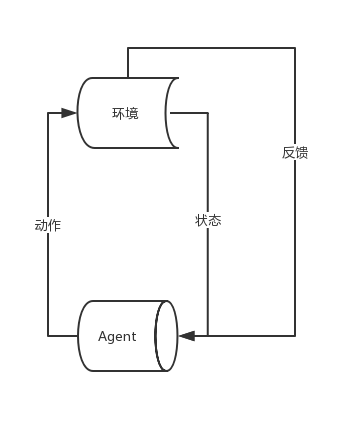
\includegraphics[scale=0.5]{static/RL.png}
  \caption{强化学习示意图}
\end{figure}
\cleardoublepage

\section{深度强化学习的发展概况
}
\subsection{传统强化学习}
传统强化学习主要分为基于价值的Q-learning\cite{Mnih2013Playing},和基于策略的Sarsa。\begin{equation}\label{eq:DQN}
  Q\left(s_{t}, a_{t}\right) \leftarrow Q\left(s_{t}, a_{t}\right)+\alpha\left[r_{t+1}+\gamma \max _{a} Q\left(s_{t+1}, a\right)-Q\left(s_{t}, a_{t}\right)\right]  
\end{equation}

Q-learning(\ref{eq:DQN})主要通过一张Q-table作为输入状态与输出动作价值的估计,通过Q-table来进行更新。
Sarsa(\ref{eq:Sarsa})是一种在线学习的算法,Q-learning是一种离线学习算法。Sarsa选取的是一种保守的策略,他在更新Q值的时候已经为未来规划好了动作,对死亡和错误比较敏感;Q-learning算法相比较而言更加大胆,Q-learing在更新的时候选取的是最大Q值的方向,对死亡和错误不敏感。
\begin{equation}\label{eq:Sarsa}
  Q\left(s_{t}, a_{t}\right) \leftarrow Q\left(s_{t}, a_{t}\right)+\alpha\left[r_{t+1}+\gamma Q\left(s_{t+1}, a_{t+1}\right)-Q\left(s_{t}, a_{t}\right)\right]
\end{equation}

\subsection{深度学习的兴起}
\begin{figure}[!htp]
  \centering
  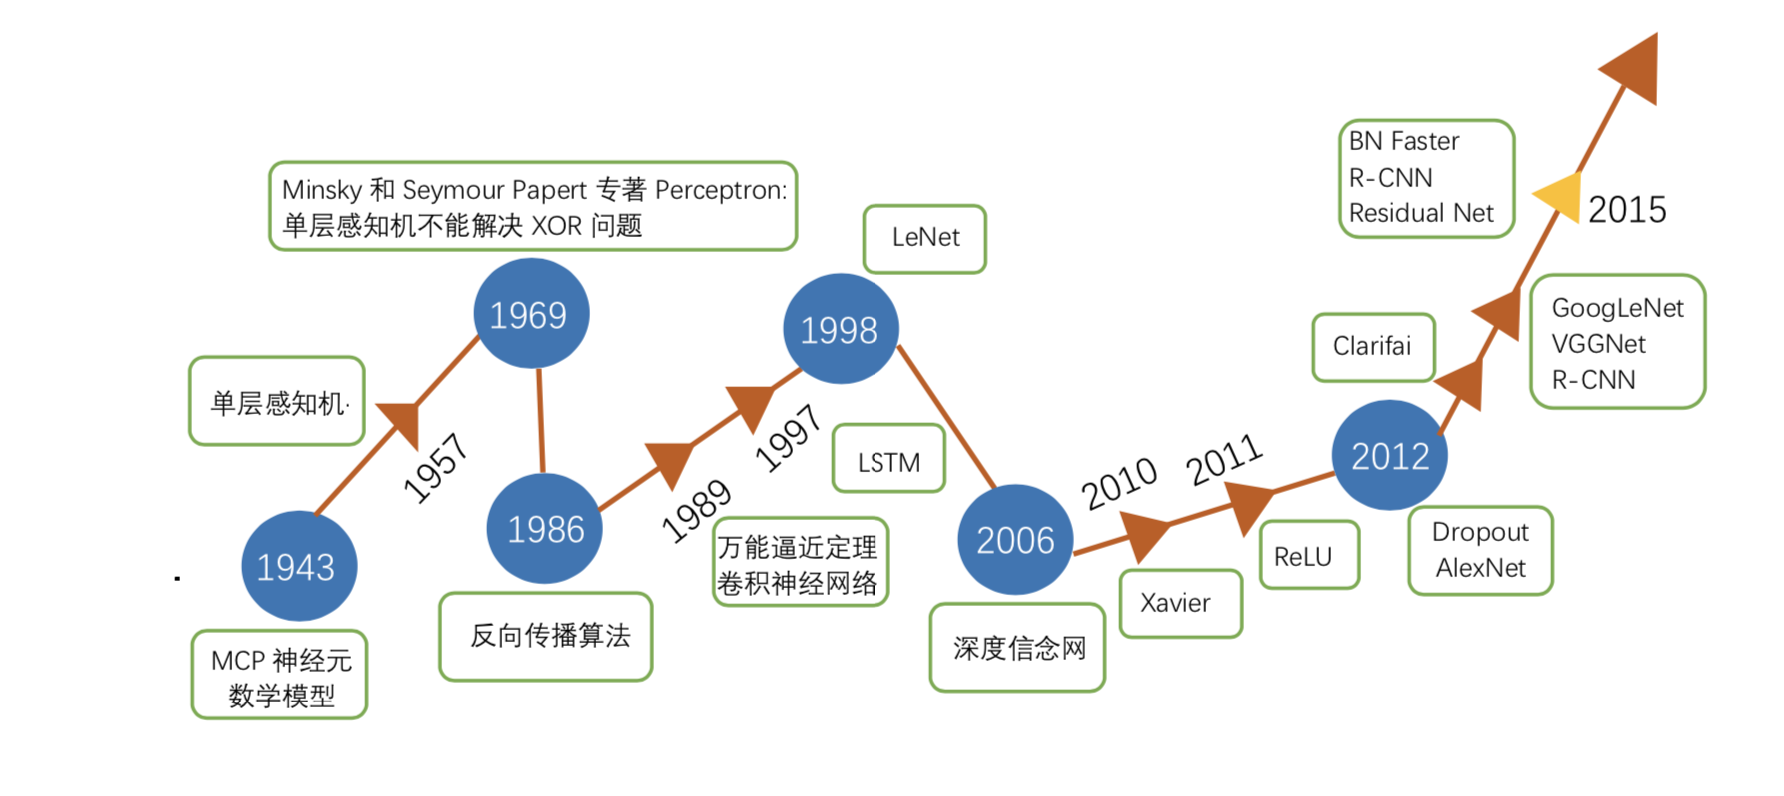
\includegraphics[scale=0.5]{static/develop.png}
  \caption{深度学习的发展}
\end{figure}
深度学习(Deep Learning:DL)这个概念在很早之前就已经提出,但是在深度学习的发展经历过数次的高潮,也经历过数次低谷,在最近几年开始重新成为热门研究话题。MCP人工神经元模型早在1943年就被提出,希望能够通过计算机来模拟人类的神经元处理输入信号的反应过程。MCP模型将神经元简化为:输入信号线性加权,求和操作,非线性函数激活(阈值法)输出。Minsky在1969年经过深入的研究,得出感知器在本质上是线性模型,只能处理线性分类问题,无法处理非线性问题\cite{Rosenblatt1958The}。在证明了感知器存在的这种局限性之后,神经网络的发展迎来持续数十年寒冬时期。适用于多层感知器(MLP)的BP(反向传播)算法\cite{rumelhart1988learning}于1989年被提出,也被称为BP神经网络。BP神经网络引入了一种特殊的激活函数Sigmoid激活函数,通过这种函数可以对神经网络进行非线性映射,有了非线性映射关系,非线性分类问题(如XOR异或问题)得到了有效解决,同时BP算法使得神经网络能进行有效地更新学习。在1989年LeCun发明了卷积神经网络Le-Net\cite{lecun1998gradient},并将其用于数字识别,虽然取得了较好的效果,但是在当时并没有引起足够的注意。1991年,BP算法被指出存在梯度爆炸或梯度消失问题,由于Sigmoid函数的饱和特性,在深层神经网络误差梯度后向传递的过程中,后层梯度以乘性方式叠加到前层,误差梯度传到前层时几乎为0,因此无法对前层进行有效的学习。2006年是深度学习元年,Hinton提出了深层网络训练中梯度消失问题的解决方案。通过无监督预训练对权值进行初始化和有监督训练微调\cite{hinton2006fast}这两种方式,能够有效解决深层神经网络训练中出现的梯度爆炸或者梯度消失的问题。2012年Hinton使用AlexNet\cite{krizhevsky2012imagenet}的神经网络结构参加ImageNet比赛,一举夺得冠军,并且大幅超越第二名传统机器学习SVM的正确率。在随后的几年中,通过ImageNet图像识别比赛。随着深度学习研究的发展以及硬件计算能力的提升,深度学习在其他领域也表现出强大的生命力。在ImageNet之后深度学习受到了广泛的关注,越来越多的深度学习研究开展,并且在不同的领域展现出其强大的学习能力。其中卷积神经网络(CNN)的提出,极大的促进了计算机在图像处理方面的发展,特别是图像识别已经达到远远超越人类的水平。
\subsection{深度强化学习发展}
由于深度学习在人工智能领域的大放异彩,2013年DeepMind的DQN\cite{Mnih2013Playing}(Deep Q-Network:深度Q网络)是将深度学习和强化学习成功结合的开端。DQN算法用一个神经网络代表价值函数,根据传统强化学习中的Q-Learning算法为神经网络提供目标值,通过网络不断更新直至收敛来学习感知和决策的能力。DQN在Atari上取得超越之前所有算法,并在其中6个游戏中取得了超越人类的成绩。DQN算法用到了两个关键技术:
\begin{enumerate*}
  \item 使用经验库打破样本间关联性;
  \item 使用固定目标网络使得训练的稳定性和收敛性更好。
\end{enumerate*}

DQN算法是整个深度强化学习研究的开山之作,引起了许多研究团队和学者的关注。DQN算法的主要改进如下表展示,其中double DQN\cite{van2016deep}、优先级经验回放(Priorized Experience Replay)DQN\cite{schaul2015prioritized}、竞争架构(Dueling-Net)DQN\cite{wang2015dueling}是DQN算法最为代表性的三大改进。在DQN算法取得很大成功之后,受到了越来越多的关注,之后有更多算法的提出,深度强化学习不断地涌现强大的生命力。
\begin{table}
  \centering
  \caption{DQN改进算法\cite{唐振韬2017深度强化学习进展}}
  \begin{tabular}{@{}llr@{}} \toprule
    年份 & 研究单位 & 算法 \\ \hline
    2015 & DeepMind & DQN \\ \hline
    2015 & DeepMind & 分布式DQN\cite{nair2015massively} \\ \hline
    2016 & DeepMind & double DQN\cite{van2016deep} \\ \hline
    2016 & DeepMind & 优先级经验回放 DQN\cite{schaul2015prioritized} \\ \hline
    2016 & DeepMind & dueling DQN\cite{wang2015dueling} \\ \hline
    2016 & Standford \& DeepMind & 引导 DQN\cite{osband2016deep} \\ \hline
    2016 & DeepMind & 异步 DQN\cite{mnih2016asynchronous} \\ \hline
    2017 & Technion & 平均 DQN \\ \hline
    2017 & Illinois Urbana-Champaign & 约束优化 DQN \\ \hline
    2017 & DeepMind & 分类 DQN \\ \hline
    2017 & DeepMind & 噪声 DQN \\ \hline
    2017 & DeepMind & Rainbow \\ \hline
  \end{tabular}
\end{table}
\section{深度强化学习研究现状}
深度强化学习的目前研究主要分为:
\begin{enumerate*}
  \item 基于价值(value based);
  \item 基于策略(policy based);
  \item 基于价值和基于策略结合的Actor-Critic算法。
\end{enumerate*}
\subsection{基于价值}
DQN是多层卷积神经网络,其输出给定状态s和网络参数$\theta$的动作值向量。它是从$R_n$到$R_m$的函数,其中n是状态空间的维度,m是动作空间的维度。 DQN算法的三个关键要素是体验重放,固定目标Q网络,以及限制奖励范围。体验重播解决了之前提出的奖励通常是延时的问题,它有助于打破数据的相关性,并从过去的所有经验中学习,存储一组最近的转换过程以用于某些预定步骤并随机均匀地采样以更新网络。
\subsection{基于策略}
基于价值的强化学习算法的基本思想是根据当前的状态,计算采取每个动作的价值,然后根据价值贪心的选择动作。策略梯度(Policy Gradient)\cite{sutton2000policy}则省略了计算每个动作的价值,而是直接根据当前的状态来选择来进行决策的算法。

策略梯度的核心思想是更新参数时有以下考虑:如果当前回合选择某一动作,那么下一回合选择执行该动作的概率大一些。执行动作完成之后再看环境的反馈,如果反馈是正的,那么就会增加执行这个动作的概率,如果反馈是负的,就会减小执行这个动作的概率。
\subsection{Actor-Critic}
Actor-Critic\cite{Barto1998Reinforcement}是将基于价值(比如DQN)和基于策略(比如Policy Gradient)两类强化学习结合起来。因此Actor-Critic分为两个部分:Actor(基于策略)和Critic(基于价值)。为了介绍这类算法,接下来举一个玩游戏的例子:

Actor(玩家):为了使这个游戏得到尽量高的分数reward(奖励),需要实现一个函数:输入状态(state,如当前的游戏画面),输出动作(action,如上下左右跳跃等)。可以采用神经网络来近似这个函数。剩下的任务就是如何训练神经网络,让它的表现更好(获得得更高的reward)。这个网络就被称为Actor。

Critic(评委):为了训练Actor,需要知道Actor的表现到底怎么样,根据表现来决定对神经网络参数的调整。这就要用到强化学习中的“Q-value(Q价值)”。Q-value也是一个未知的函数,也可以用神经网络来近似。这个网络被称为critic。

Actor和Critic之间协调工作的过程:
\begin{enumerate}
  \item Actor看到游戏目前的状态,做出一个动作。
  \item Critic根据状态和动作两者,对Actor刚才的表现打一个分数。
  \item Actor依据critic的打分,调整自己的策略(Actor神经网络参数),争取下次做得更好。
  \item Critic根据环境给出的真实reward和其他评委的打分(Critic target网络输出的分数)来调整自己的打分策略(Critic神经网络参数)。
  \item 一开始Actor随机表演,Critic随机打分。但是由于reward是环境所给出的真实值,Critic不断更新参数,评分越来越准,Actor表现越来越好。
\end{enumerate}

2016年DeepMind提出DDPG\cite{Lillicrap2015Continuous}(Deep Deterministic Policy Gradient)。DDPG是DPG(Deterministic Policy Gradient)的改进,是将神经网络与DPG相结合而形成的改进算法,是一种策略学习的方法。具体来说,DDPG将DPG的策略函数和Q函数使用卷积神经网络代替模型,然后使用深度学习的方法来训练上述神经网络。
其中Q函数的实现和训练方法采用了DQN算法 ,同时也是Alpha Go使用的Q函数方法。

Asynchronous Advantage Actor-Critic\cite{mnih2016asynchronous}, 简称 A3C。
A3C引入了并行计算的概念,为了训练一对Actor 和 Critic,将Actor 和 Critic 复制成多份,然后放在不同的核中进行并行训练。需要声明一个全局的Actor-Critic,多个副本并行计算更新参数传递给全局Actor-Critic,同时全局Actor-Critic也会将参数更新给这些副本。通过A3C这种方法可以有效解决Actor-Critic不收敛的问题,并行中的副本们互相独立不会产生干扰,而全局参数由所有副本提交进行更新改进,副本不会对全局参数产生连续性的干扰,从而达到降低更新的相关性、提高收敛性的效果。

PPO(Proximal Policy Optimization)\cite{schulman2017proximal} 是OpenAI 提出的一种解决 Policy Gradient 不好确定学习率 (或者步数大小) 的问题. 因为如果步数过大, 学出来的 策略 会一直乱动, 不会收敛, 但如果 步数太小, 对于完成训练,需要等待的时间太长。 PPO 利用 New Policy 和 Old Policy 的比例, 限制了 New Policy 的更新幅度, 让 Policy Gradient 对稍微大点的 步数 不那么敏感。
强化学习与监督学习有很大的差异性,相比于监督学习,强化学习想要取得预期的效果十分困难。大部分的强化学习任务在逻辑控制方面都比较复杂,且将理论应用到任务中并取得比较好的效果经过重重困难,如超参数的调整,程序的调试,损失函数梯度下降不容易实现等都要花费大量的时间与精力。而PPO采取了一系列约束条件,使得人工不需要进行大量的操作就能实现预期比较好的效果,是一种更加适合应用到实际生活过程中的算法。PPO算法在学习过程中能找到合适的更新步长,使得每次回报的函数能够单调减,也就是学习的效果不会变差。

DPPO(Distributed PPO)\cite{heess2017emergence}相比于PPO来说就是在工程方面的改进,是一种分布式训练PPO的方法。和A3C采用类似的做法,开启多线程分别和环境交互学习,不同线程学习到不同阶段的梯度计算,当所有的线程完成计算后更新全局的参数,按照这样的步骤进行迭代计算学习。

\chapter{DQN算法及其三大改进}
\section{Q-learning}
\subsection{马尔科夫决策过程}
\begin{defn}[马尔科夫性]
  当一个随机过程在给定现在状态及所有过去状态情况下,其未来状态的条件概率分布仅依赖于当前状态。A state $S_t$ is Markov if and only if :
  \begin{equation}
    P[S_{t+1}|S_t]=P[S_{t+1}|S_1,...,S_t]
  \end{equation}
\end{defn}

\begin{defn}[马尔科夫过程]
  马尔科夫过程即具有马尔科夫性的过程,即过程的条件概率仅仅与系统的当前状态相关,与它的未来或者过去历史都是独立不相关的。
\end{defn}
\begin{defn}[马尔科夫奖赏过程]
  相比于马尔科夫过程,马尔科夫奖赏过程(MRP)新增了转换过程中的奖赏函数,可以用四元组$<S,P,R,\gamma>$表示。
  \begin{itemize}
    \item $S$:有限状态的集合。
    \item $P$:表示不同状态之间相互进行转换的关系,可以用公式$P_{ss'}=P[S_{t+1}=s'|S_{t}=s]$来表示。
    \item $R$:奖赏函数。
    \item $\gamma$:折扣系数(discount factor)客观反映了更加看重眼前利益的特点,其中$\gamma$的范围为0~1闭区间。
  \end{itemize}
  \begin{defn}[奖赏函数]
    在$t$时刻的奖赏值$G_t$:
    \begin{equation}      
      G_t=R_{t+1}+\gamma R_{t+2}+...=\sum_{k=0}^\infty \gamma^k R_{t+k+1}
    \end{equation}
  \end{defn}
\end{defn}

为什么需要折扣系数$\gamma$:
\begin{itemize}
  \item 方便数学表达。
  \item 避免陷入无限循环。
  \item 长远利益有不确定性。
  \item 立即的回报相对于延迟的回报能获得更多利益。
  \item 符合人类更看重眼前利益的特点。
\end{itemize}
\begin{defn}[价值函数]
  状态$s$的长期价值函数表示为:
  \begin{equation}
    v(s)=E[G_t|S_t=s]
  \end{equation}
\end{defn}

\begin{defn}[马尔科夫决策过程]
  相比于马尔科夫奖赏过程,马尔科夫决策过程(Markov Decision Process,MDP)新增了在状态s下执行动作的决策函数,MDP可以使用五元组$<S,A,P,R,\gamma>$来表示。
  \begin{itemize}
    \item $S$:有限状态的集合。
    \item $A$:有限动作的集合。
    \item $P$:表示不同状态之间相互进行转换的关系,可以用$P_{ss^{'}}^a=P[S_{t+1}=s^{'}|S_t=s,A_t=a]$来表示。
    \item $R$:奖赏函数。
    \item $\gamma$:折扣系数(discount factor)客观反映了更加看重眼前利益的特点,其中$\gamma$的范围为0~1闭区间。
  \end{itemize}
\end{defn}

\begin{defn}[策略]
  给定状态下的动作概率分布:
  \begin{equation}
    \pi(a|s)=P[A_t=a|S_t=a]
  \end{equation}  
\end{defn}
\begin{defn}[状态价值函数]
  在处于某一环境中,机器自身的策略$\pi$的情况下,当机器在环境中处于状态s时,此时s自身存在一个价值,可以用价值函数来表示:
  \begin{equation}
    v_{\pi}(s)=E_{\pi}[G_t|S_t=s]
  \end{equation}
\end{defn}
\begin{defn}[最优状态价值函数]
  在处于某一环境中,机器自身的策略$\pi$的情况下,当机器在环境中处于状态s时,此时s自身存在的最优状态价值函数为:
  \begin{equation}
    v_{*}(s)=\max_{\pi}v_{\pi}(s)
  \end{equation}
\end{defn}
\begin{defn}[动作价值函数]
  在处于某一环境中,机器自身的策略为$\pi$、环境当前的状态为$s$的情况下,机器执行某一动作$a$会产生一定量的价值,这种价值和策略、状态、动作的关系可以表示为:
  \begin{equation}
    q_{\pi}(s,a)=E_{\pi}[G_t|S_t=s,A_t=a]
  \end{equation}
\end{defn}
\begin{defn}[最优动作价值函数]
  状态$s$下采取动作$a$的最优动作价值函数:
  \begin{equation}
    q_{*}(s,a)=\max_{\pi}Q_{\pi}(s,a)
  \end{equation}
\end{defn}
\begin{defn}[最优策略]
  如果策略$\pi$优于策略$\pi^{'}$:
  \begin{equation}
    \pi \geq \pi^{'} , if: v_{\pi}(s) \geq v_{\pi^{'}}(s),\forall_{s}
  \end{equation}
    
\end{defn}

\subsection{Q-learning}
对于任何马可尔夫决策过程,Q-learning\cite{Mnih2013Playing}是当前状态的最佳策略。
Q-learning通过Q估计进行决策,通过Q现实进行更新。
\begin{defn}[Q 估计]
  在当前状态s下做出动作a后到达的状态s\_获得的奖励的估计值。
\end{defn}
\begin{defn}[Q 现实]
  在当前状态s下做出动作a后到达状态s\_获得的奖励的实际值。
\end{defn}
\begin{defn}[Q 表]
  当机器在环境中处于不同的状态$s_i$下,执行不同的动作$a_j$时,会产生不同且唯一确定的价值Q,把所有的状态与执行动作的组合得到的价值列成一张表格,称之为Q表(Q-table)。
  \begin{table}
    \begin{center}
      \caption{Q-table}
      \begin{tabular}{|l|c|r|} 
        \hline
        Q-table & $a_1$ & $a2$ \\ 
        \hline
        $s_1$ & $Q(s_1,a_1)$ & $Q(s_1,a_2)$ \\ 
        \hline
        $s_2$ & $Q(s_2,a_1)$ & $Q(s_2,a_2)$ \\ 
        \hline
        $s_3$ & $Q(s_3,a_1)$ & $Q(s_3,a_2)$ \\ 
        \hline
      \end{tabular}
      
    \end{center}
  \end{table}
  
\end{defn}
Agent(玩家)进入每个状态$s_i$时,通过查阅Q表,能得到在$s_i$时选择不同动作$a_i$的期望值(Q 估计)$Q(s_i,a_i)$,选择其中最大的Q值所对应的动作,会进入不同的状态$s_j$,同时环境会给agent一个回报reward(Q 现实)。
\begin{cor}[Q-learning]
  根据以上推导,可以对Q值计算,也就是Q\_table更新过程,其中$\alpha$为学习率,$\gamma$为奖励性衰变系数。
  \begin{equation}
    Q\left(S_{t}, A_{t}\right) \leftarrow Q\left(S_{t}, A_{t}\right)+\alpha\left[R_{t+1}+\gamma \max _{a} Q\left(S_{t+1}, a\right)-Q\left(S_{t}, A_{t}\right)\right]
  \end{equation}
\end{cor}
\begin{exmp}[挖宝藏小游戏]
  
  O - - - - T

  在这个例子中,O代表agent,T代表宝藏,一开始宝藏在最右边,agent在最左边,在每一步动作中,agent可以选择两个动作,left(向左走)或者right(向右走)。

  例如,在这个过程中的某个状态为:

  - O - - - T

  接下来Agent可以选择
  \begin{itemize}
    \item left:O - - - - T
    \item right:- - O - - T
  \end{itemize}

  我们可以用O所在的位置(0,1,2,3,4,5)表示agent所在的状态,当agent比上一个状态更加靠近宝藏的时候,我们(环境)给agent一个正反馈(reward>0),当agent比上一步远离agent的时候,我们给agent一个负反馈(reward<0)。

  那么此时的Q表为如下形式:
  \begin{table}
    \begin{center}
      \caption{挖宝藏小游戏 Q-table}
      \begin{tabular}{|l|c|r|}
        \hline
        $Q-table$ & left & right \\
        \hline
        0 & q(0,left) & q(0,right) \\
        \hline
        1 &q(1,left) &q(1,right) \\
        \hline
        2 &q(2,left)  &q(2,right) \\
        \hline
        3 &q(3,left) &q(3,right) \\
        \hline
        4 &q(4,left) &q(4,right) \\
        \hline
        5 &q(5,left) &q(5,right) \\
        \hline
      \end{tabular}
    \end{center}
  \end{table}

  当Agent在i位置的时候,当Agent选择$right$,Agent将会靠近宝藏,那么Agent将会获得环境的正反馈$r_i$,那么对应的$Q(i,right)$将会增加$r_i$;如果Agent选择$left$,那么Agent会远离宝藏,环境会给Agent一个负反馈$r_i$,那么对应的$Q(i,right)$将会减少$r_i$。

\end{exmp}

通过智能体(Agent)、环境(environment)、奖励(reward)、动作(action),状态(state)这五个要素可以将问题抽象成一个马尔科夫决策过程,我们在每个格状态$s_t$可以根据Q\_table选择一个动作执行,得到环境状态的反馈同时进入下一个状态$s_{t+1}$,根据环境反馈的状态更新Q\_table。
\cleardoublepage
\begin{algorithm}
  \caption{Q-learning}
  \label{Q-learning}
  \begin{algorithmic}[1]
    \State {初始化$Q-table$}
    \For{回合 $in$ 所有回合}
    \State 初始化状态s
    \For{步骤 $in$ 本回合所有步骤}
    \State 使用$Q-table$在当前状态$s$所有可以选择的$action$中,选取$Q$值最大的动作$a$
    \State 执行动作$a$,获得环境反馈的奖励值$r$,并进入新的状态$s^{'}$
    \State 更新$Q-table$ : $$Q\left(S_{t}, A_{t}\right) \leftarrow Q\left(S_{t}, A_{t}\right)+\alpha\left[R_{t+1}+\gamma \max _{a} Q\left(S_{t+1}, a\right)-Q\left(S_{t}, A_{t}\right)\right]$$
    \State $s \gets s'$
    \EndFor
    \EndFor
  \end{algorithmic}
\end{algorithm}

传统强化学习Q-learning算法通过一张Q-table不断探索和更新Q值,计算出agent最佳的选择。Q-table必须把agent可能遇到的每一个状态都存下来,那么在面对如电子游戏这样的复杂游戏下,状态数量过多,Q-table将会大到无法想象,计算机无法存储如此大表格。因此传统强化学习Q-learning无法处理这样的复杂环境。
\section{卷积神经网络}
深度学习自从2006年以来受到了广泛的关注,目前深度学习已经成为大数据(Big Data)和人工智能(AI)的一个研究热点。通过建立起类似于人脑的神经网络结构,深度学习神经网络可以提取出输入数据从低层次到高层次的特征,很好的建立起了底层原始输入信号到高层语义理解的映射关系。
深度学习可以表示多层次抽象的数据(如知识图谱,词向量),用来提供给不同的计算模型进行学习任务。深度学习这种方法在许多领域都引领了发展,包括最先进的语音识别、计算机视觉对象识别、对象检测和许多其它领域如医疗领域等。大数据中的复杂结构可以通过深度学习来进一步挖掘和发现,BP算法能够指导计算机从后面的神经网络层传递误差到前面的神经网络层来改变本层的参数。在计算机视觉领域的处理、语音合成、音频处理等方面,深度学习已经有了较为成熟的工业应用,而神经网络中的一种网络结构递归网络,在文本和语音等处理序列的方面展现了强大的能力。
\subsection{基本概念}
\begin{defn}[人造神经元(Neuron)]
  类似于人类大脑的基本单元,大量的神经元排列组合构成了神经网络。在神经网络中,神经元接收输入数据,经过神经元的处理得到输出,而这个输出被发送到其他神经元用于进一步处理,或者作为最终输出进行输出。 
  一般神经元包含:
  \begin{itemize}
    \item 输入:神经元的输入数据;
    \item 权重:当输入进入神经元时,它会乘以一个权重;
    \item 偏差:改变权重与输入相乘所得结果的范围;
    \item 激励函数:决定了当前神经元是否达到激活状态,通常为非线性函数如Sigmoid,Relu等;
    \item 输出:神经元的输出数据。
  \end{itemize}
  数学表示:$t=f(W*A+b)$,W为权重向量,A为输入向量,b为偏置,f为激励函数,t为输出。
  
\end{defn}
\begin{figure}[ht]
  \centering
  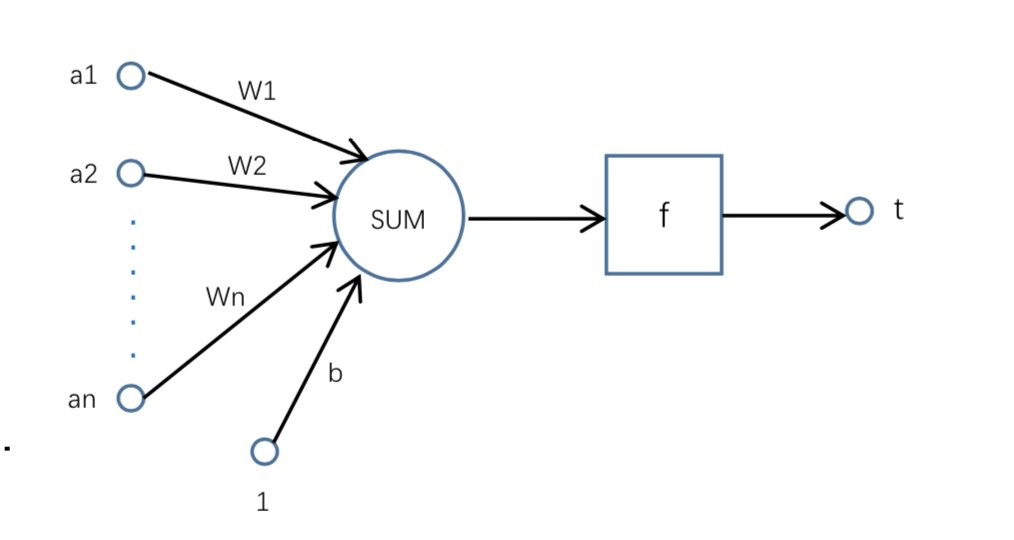
\includegraphics[scale=0.4]{static/Ncell.png}
  \caption{人造神经元}
\end{figure}

\begin{defn}[神经网络]
  神经网络是由大量神经元经过不同的排列组合而形成,不同的神经元之间之间传递相互数据,通过BP算法来不断调整自身的参数。神经元具有激活阈值,相当于神经元激活的最低要求值,如果神经元的权重值的组合和传递给它的数据之和大于等于这个阈值的话,将会导致神经元产生激活,神经元的组合可以产生学习的能力。
  典型的人工神经网络具有以下三个部分:
  \begin{itemize}
    \item 结构,结构指定了网络中的变量和它们的拓扑关系;
    \item 激励函数,定义了神经元改变自身状态(是否激活)的规则,如果激活就可以将数据传递到下一层,一般是一个非线性函数;
    \item 学习规则,学习规则指定了网络中的权重参数如何随着时间推进而进行相应的调整。
  \end{itemize}
  
\end{defn}

\begin{figure}
  \centering
  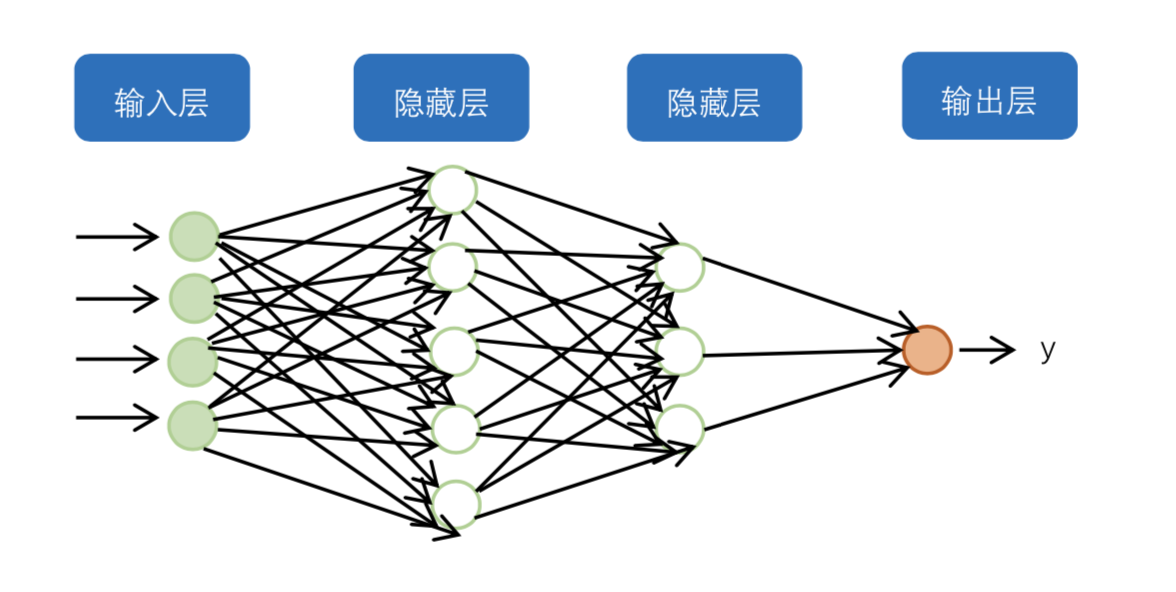
\includegraphics[scale=0.5]{static/network.png}
  \caption{普通神经网络}
\end{figure}

\begin{defn}[输入层]
  接受输入的那一层,本质上是网络的第一层;
\end{defn}
\begin{defn}[输出层]
  生成输出的那一层,本质上是网络的最后一层;
\end{defn}
\begin{defn}[隐藏层]
  处理输入层传入的信号的中间若干层的神经网络,隐藏层根据不同的任务做不同的处理得到中间输出数据,传递到下一层。
\end{defn}
\subsection{多层神经网络}
\begin{defn}[MLP(多层感知器)]
  单个神经元能执行的任务(函数)复杂度有限,类似于CPU中的门结构,使用大量神经元进行堆栈组合可以实现复杂任务的处理输出。一个输入层、一个隐藏层和一个输出层可以构成最简单的神经网络。每个层都有多个神经元,并且每个层中的所有神经元都连接到下一层的所有神经元。这些网络也可以被称为完全连接的网络。 
\end{defn}
多层神经网络的学习过程
\begin{enumerate}
  \item 从输入层开始,原始输入数据通过神经网络向前传递,数据经过不同层次的处理得到输出结果;
  \item 基于网络的输出,通过损失函数得到目标与当前数据的误差;
  \item 反向计算这个误差,计算误差相对于网络中每个权值参数的导数,更新模型的参数。
\end{enumerate}
2006年,深度学习的经典文章《Reducing the dimensionality of data with neural networks》\cite{hinton2006reducing}提出了如下的主要观点:
\begin{enumerate*}
  \item 多层神经网络具有更加优异的特征学习能力;
  \item 通过逐层初始化可以有效克服多层神经网络更新学习的困难。
\end{enumerate*}

\subsection{卷积神经网络}

卷积神经网络(Convolutional Neural Networks, CNN)是一种特殊的神经网络结构,包含了若干个卷积层和池化层,以此完成对原始数据特征的抽取。不同于普通神经网络中的全连接,在卷积层中,一个神经元只与部分相邻网络层中的神经元进行连接。通过卷积和子采样(池化)两个操作可以大大简化模型复杂度,减少模型需要调整的参数。
\begin{figure}[h]
  \centering
  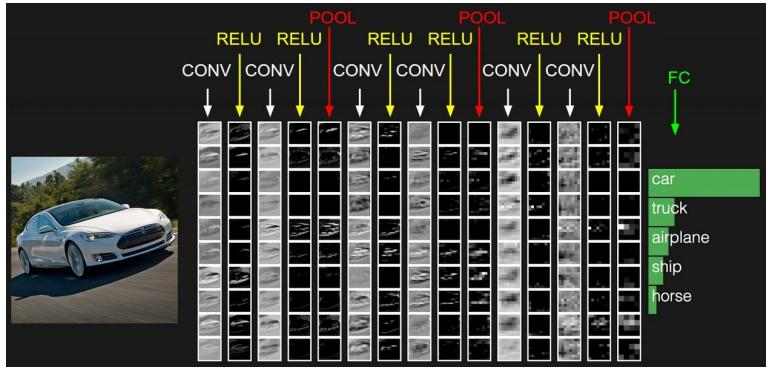
\includegraphics[scale=0.5]{static/cnn.jpg}
  \caption{典型卷积神经网络结构\cite{CNN2017}}
\end{figure}
卷积神经网络是传统神经网络的一个改进,在普通层级神经网络的基础上对不同层的功能和形式做出了一些改变。
卷积神经网络的一般结构:
\begin{enumerate}
  \item 数据输入层/ Input layer
  \item 卷积计算层/ CONV layer
  \item 激励函数层 / ReLU layer
  \item 池化层 / Pooling layer
  \item 全连接层 / FC layer
\end{enumerate}


数据输入层主要是对原始图像数据进行预处理,其中包括:
\begin{itemize}
  \item 去均值操作:为了把样本的中心拉回到坐标系原点上,对输入的原始数据在各个维度上都中心化为0;
  \item 归一化: 为了减少各个维度数据取值差异带来的干扰,将不同维度的数据范围归一化相同的范围,如将原始所有的数据归一化到[-1,1]的范围;
  \item 白化:相当于在数据的特征轴上对数据做归一化。
\end{itemize}

卷积层是卷积神经网络最重要的一个层次,
在卷积层中,有两个关键操作:
\begin{itemize}
  \item 窗口滑动,滤波器对局部数据进行计算,提取出数据的局部特征;
  \item 局部关联,将神经元视为滤波器,使用神经元对原始数据做滤波操作。 
\end{itemize}

卷积神经网络采用的激励函数一般为ReLU(The Rectified Linear Unit,修正线性单元),通过这样的非线性函数可以将卷积层的输出结果做非线性映射。
采取Relu可以加速网络的收敛,方便求网络的梯度,函数的图像如(\ref{fig:Relu})所示:
\begin{figure}[h]
  \centering
  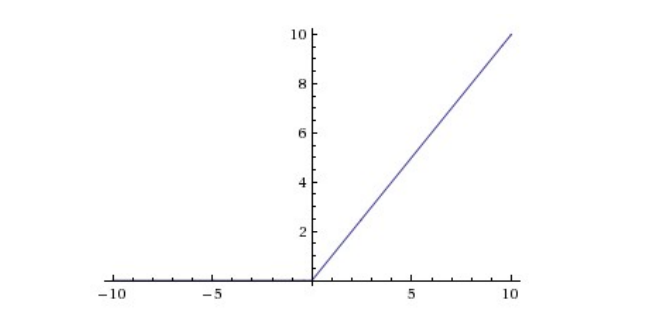
\includegraphics[scale=0.5]{static/Relu.png}
  \caption{Relu函数图像}
  \label{fig:Relu}
\end{figure}

为了压缩数据和减少参数的数量,减小神经网络过拟合的风险,可以通过池化操作完成。池化层位于连续的卷积层中间,
具体来说,如果输入是图像数据的话,那么池化层的最主要作用就是压缩图像的大小。

卷积神经网络尾部一般用全局连接层来进行连接过渡,和普通的神经网络神经元的连接方式完全相同。全连接层一般用于得出神经网络最后的输出结果。
\section{DQN算法}
伴随着深度学习的发展,深度学习也在传统强化学习产生重要的应用,DQN(deep Q network)就是一种融合了深度学习与强化学习的方法。

2015年DeepMind在文章《Playing Atari with Deep Reinforcement Learning》\cite{mnih2013playing}提出了DQN ,DQN是第一个直接从图像的原始像素中成功学习到控制策略的深度强化学习算法。DQN使用卷积神经网络代替Q-learning中的价值函数,对机器当前状态应选的动作输出相应的动作价值。因此DQN算法的决策核心就是卷积神经网络,DQN的输入为原始图像像素,输出为当前状态的价值函数,训练采用Q-learning的方法来进行。DQN算法应用到Atari2600的许多游戏上,取得很大的成功,有的甚至达到了超越人类最高分的水平。

之后DeepMind在Nature上发表了改进版的DQN文章\cite{mnih2015human},引起了广泛的关注,深度强化学习从此成为深度学习领域的前沿研究方向与研究热门。

将深度学习应用在强化学习上,面临诸多挑战。大部分深度学习算法需要巨大的训练数据量,但传统强化学习提供的数据通常比较稀疏,噪声也很大,通常在执行完动作不能立即获得奖励;强化学习获得的回报与产生这个结果的动作可能会有很长的间隔,各个相邻的状态之间有很强的关联性,而深度学习一般假设样本数据独立进行分布。就是,随着训练的进程,价值函数对动作价值的估计不断得到优化。而随着价值函数的变化,其Q值输出(动作输出)也会跟着改变,继而产生的训练样本的分布也会改变,这与深度学习要求训练用的数据分布不变不符合。

DQN不用Q表记录Q值,而是用神经网络来预测Q值,并通过不断更新神经网络从而学习到最优的行动路径。
DeepMind 用DQN来玩电子游戏,他们将游戏画面的像素转换成深度神经网络的输入数据(状态s),用CNN(卷积神经网络)来预测动作a($a_1$,$a_2$,$a_3$ ....), 和对应的Q(s, $a_1$), Q(s, $a_2$),Q(s, $a_3$)...
然后算法通过更新神经网络(NN)中的参数(w, b ...),来更新NN,从而优化模型得到最优解。

为了使训练的样本之间不会相互依赖,DQN设置了一个经验库用来存放以前不同状态之间的转换关系的数据,然后每次在经验库中经过随机采样得到训练所需的数据样本;采用过去的多个样本做平均,训练样本分布得到平滑,使得样本分布变化的问题得到减缓。
在经验回放过程中,将多个回合转化过程中,机器每一步使用神经网络贪心地选择动作,产生的经验$e_t = <s_t, a_t, r_t, st+1>$,存入一个经验记忆池D中。在算法参数更新的操作中,对记忆池里的样本数据进行随机采样或批量随机采样,通过Q-learning算法对模型进行参数更新。由于神经网络无法处理边长的原始数据,因此DQN使用固定长度的历史数据表示状态,例如过去连续若干图像帧的排列。

DQN这种方法对于传统的在线Q-learning来说,具有以下优势:
\begin{itemize}
  \item 通过多次采样每一步的数据,很大程度上提高了数据的利用效率。
  \item 通过随机采样打破了从连续数据里学习效率低下的问题,降低更新参数的方差。
  \item 通过在经验库中随机采样,可以得到平均分布的各个状态下的数据,解决了训练会产生发散的问题。
\end{itemize}

\begin{figure}[h]
  \centering
  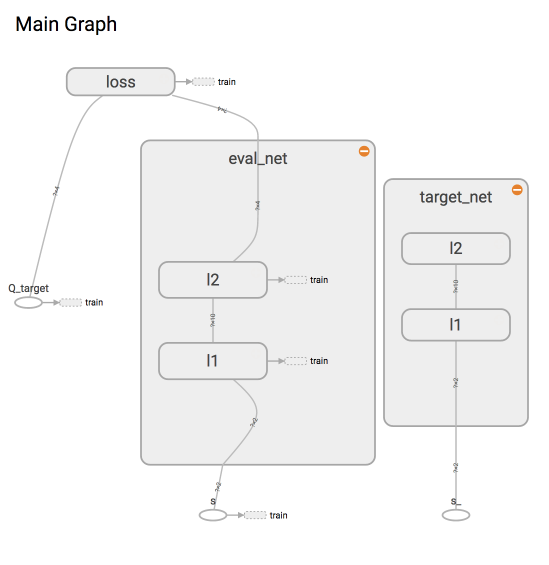
\includegraphics[scale=0.5]{static/dqn.png}
  \caption{DQN网络结构}
\end{figure}
DQN中的损失函数定义为:
\begin{equation}
  \label{DQN:loss}
  L_{i}\left(\theta_{i}\right)=\mathbb{E}_{s, a \sim \rho(\cdot)}\left[\left(y_{i}-Q\left(s, a ; \theta_{i}\right)\right)^{2}\right]
\end{equation}


DQN中有两个神经网络。一个参数相对固定的网络,我们叫做target-net,用来获取Q-目标(Q-target)的数值, 另外一个叫做eval-net用来获取Q-评估(Q-eval)的数值。
我们在训练神经网络参数时用到的损失函数(Loss function),实际上就是q\_target 减 q\_eval的结果 (loss = q\_target- q\_eval )。
反向传播真正训练的网络是只有一个,就是eval\_net。target\_net 只做正向传播得到q\_target $(q\_target = r +\gamma*max Q(s,a))$. 其中 Q(s,a)是若干个经过target-net正向传播的结果。

训练的数据是从记忆库中随机提取的,记忆库记录着每一个状态下的行动,奖励,和下一个状态的结果$<s, a, r, s^{'}>$。记忆库的大小有限,当记录满了数据之后,下一个数据会覆盖记忆库中的第一个数据,记忆库就是这样覆盖更新的。
q\_target的网络target\_net也会定期更新一下参数,由于target\_net和eval\_net的结构是一样的。更新q\_target网络的参数就是直接将q\_eval 的参数复制过来。
\cleardoublepage
\begin{algorithm}
  \caption{DQN算法}
  \begin{algorithmic}
    \State 初始化检验回放库D大小为N
    \State 初始化Q网络参数
    \For{i in range(回合总数M)}
    初始化状态$s_1=\{x_1\}$,并预处理$\phi_1=\phi\{s_1\}$
    \For{t in range(T)}
    \State 通过概率分布为$\epsilon$ 的概率,选取当前一个动作$a_t$
    \State 否则选取动作$a_t=\max_a Q^* (\phi(s_t),a;\theta)$
    \State 执行动作$a_t$,并获得获得环境给的反馈$r_t$,进入新的画面$x_{t+1}$
    \State 设置$s_{t+1}=s_t,a_t,x_{t+1}$并且处理$\phi_{t+1}=\phi(s_{t+1})$
    \State 将$(\phi_t,a_t,r_t,\phi_{t+1})$存储到经验库D中
    \State 从经验库D中随机抽取转换关系$(\phi_j,a_j,r_j,\phi_{j+1})$
    \If{$\phi_{j+1}$时刻游戏结束}
    \State $y_j=r_j$
    \Else
    \State $y_j=r_j+\gamma \max_{a^{'}}Q(\phi_j,q_j;\theta)$
    \EndIf
    \State 实施梯度下降更新网络参数,$loss=(y_j-Q(\phi_j,a_j;\theta))$
    \EndFor
    \EndFor
  \end{algorithmic}
\end{algorithm}

\section{DQN三大改进}
\subsection{double DQN}
double DQN\cite{van2016deep,hasselt2010double}的改进是关于DQN的公式的改进。
根据上面的损失函数(\ref{DQN:loss}),$y_i$也被我们称为q-target值,而后面的Q(s,a)我们称为q-eval值,我们希望q-target和q-eval值越接近越好。

q-target计算的公式:
\begin{equation}
  Y_{t}^{\mathrm{Q}} \equiv R_{t+1}+\gamma \max _{a} Q\left(S_{t+1}, a ; \boldsymbol{\theta}_{t}\right)
\end{equation}
进一步展开:
\begin{equation}
  Y_{t}^{\mathrm{Q}}=R_{t+1}+\gamma Q\left(S_{t+1}, \underset{a}{\operatorname{argmax}} Q\left(S_{t+1}, a ; \boldsymbol{\theta}_{t}\right) ; \boldsymbol{\theta}_{t}\right)
\end{equation}

也就是说,我们根据状态$s^{'}$选择动作$a^{'}$的过程,以及估计Q($s^{'}$,$a^{'}$)使用的是同一张Q值表,或者说使用的同一个网络参数,这可能导致选择过高的估计值,从而导致过于乐观的值估计。

为了避免这种情况的出现,我们可以对选择和衡量进行解耦,从而就有了doubel DQN,在Double DQN中,q-target的计算基于如下的公式:
\begin{equation}
  \label{alg:double-dqn}
  Y_{t}^{\text { DoubleQ }} \equiv R_{t+1}+\gamma Q\left(S_{t+1}, \operatorname{argmax}_{a} Q\left(S_{t+1}, a ; \boldsymbol{\theta}_{t}\right) ; \boldsymbol{\theta}_{t}^{\prime}\right)
\end{equation}

我们根据一张Q表或者网络参数来选择我们的动作$a^{'}$,再用另一张Q值表活着网络参数来衡量Q($s^{'}$,$a^{'}$)的值。
\subsection{Prioritized Experience Replay DQN}
Prioritized Experience Replay DQN\cite{,schaul2015prioritized} 是关于DQN在经验回放的改进。
对于增强学习过程中,agent在一系列的动作选择中得到的经验,存在很大的相关性,这违反了常见的梯度下降算法对于样本的假设。同时对于一些出现几率很小,但是可能很有用的经验,忘记得非常快。
经典DQN在经验回放学习时采取均匀采样的方法,那么当一个agent在学习过程中,遇到的正例很少,负例很多的类似正反馈负反馈样本及其不均衡的时候,那么agent每一次回放学习到的东西就会非常少,学习效率就会变得十分低下。

DQN使用了experience replay(经验回放)来克服这些困难。
对于prioitization(优先级),重要的是如何衡量经验的重要性。作者选择了TD-error(\ref{TD-error})(Temporal-Difference error,时序差分-error)。它直观地解释是:agent对这个经验的惊讶程度,也就是有多超乎意料。
如果 TD-error 越大, 就代表我们的预测精度还有很多上升空间, 那么这个样本就越需要被学习, 也就是优先级 p 越高.
TD-error:
\begin{equation}\label{TD-error}
  \delta_{t} :=R_{t}+\gamma_{t} \max _{a} Q\left(S_{t}, a\right)-Q\left(S_{t-1}, A_{t-1}\right)
\end{equation}
在这篇论文中,作者提出来优先选择那些对于训练更加有效的经验,而不是DQN中的随机提取经验进行学习。因为,对于一个agent来说,某些经验会比其他经验更加有用,对于那些TD-error更大的经验,给予更多的检验回放的机会。

有了 TD-error 就有了优先级 p, 那我们如何有效地根据 p 来抽样呢? 如果每次抽样都需要针对 p 对所有样本排序, 这将会是一件非常消耗计算能力的事。因此需要采取另一种方法, 这种方法不会对得到的样本进行排序。这种抽样方法就叫做SumTree。
\begin{figure}[h]
  \centering
  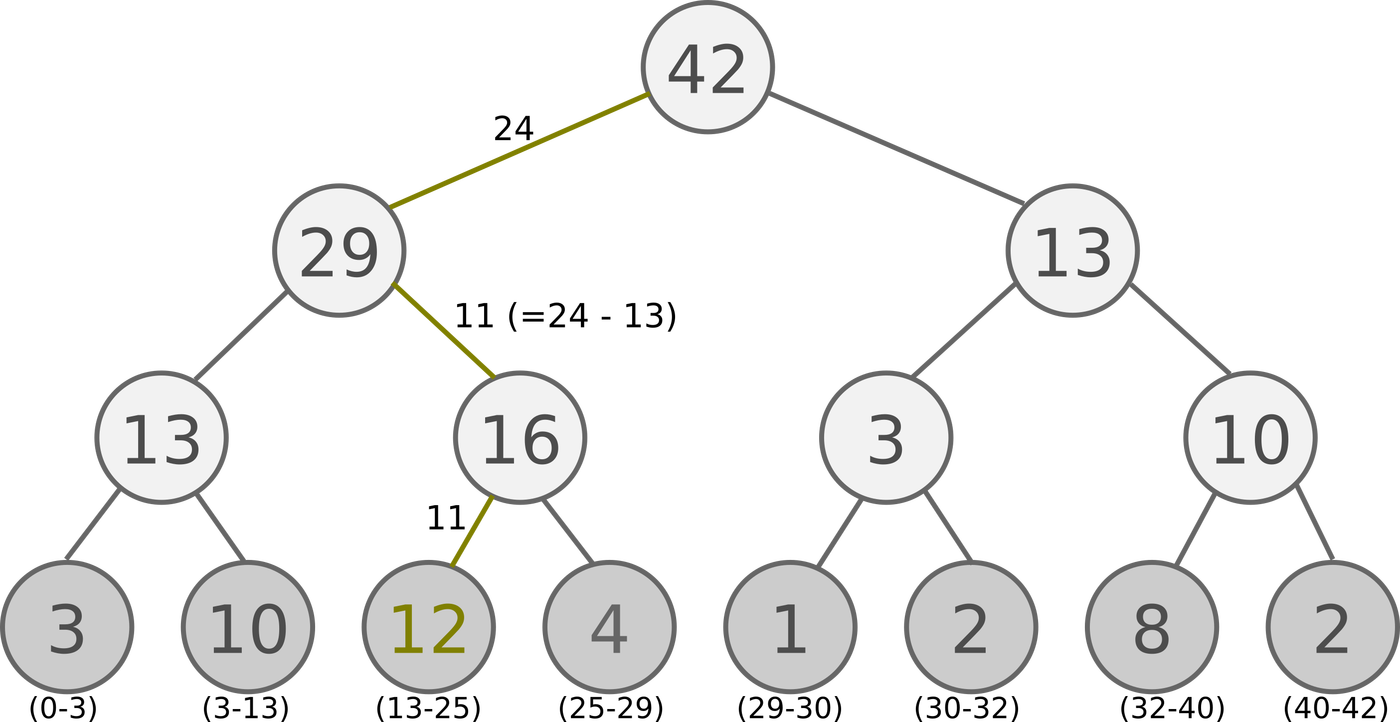
\includegraphics[scale=0.5]{static/sum_tree.png}
  \caption{SumTree}
\end{figure}
SumTree 是一种树形结构, 每片树叶存储每个样本的优先级 p, 每个树枝节点只有两个分叉, 节点的值是两个分叉的合, 所以 SumTree 的顶端就是所有 p 的合. 最下面一层树叶存储样本的 p, 叶子上一层最左边的 13 = 3 + 10, 按这个规律相加, 顶层的 root 就是全部 p 的和。

抽样时, 我们会将 p 的总合 除以 batch size, 分成 batch size 那么多区间, (n=sum(p)/batch\_size)。如果将所有 node 的 priority 加起来是42的话, 我们如果抽6个样本, 这时的区间拥有的 priority 可能是这样:
$$[0-7], [7-14], [14-21], [21-28], [28-35], [35-42]$$

然后在每个区间里随机选取一个数. 比如在第区间 [21-28] 里选到了24, 就按照这个 24 从最顶上的42开始向下搜索. 首先看到最顶上 42 下面有两个 child nodes, 拿着手中的24对比左边的 child 29, 如果 左边的 child 比自己手中的值大, 那我们就走左边这条路, 接着再对比 29 下面的左边那个点 13, 这时, 手中的 24 比 13 大, 那我们就走右边的路, 并且将手中的值根据 13 修改一下, 变成 24-13 = 11. 接着拿着 11 和 13 左下角的 12 比, 结果 12 比 11 大, 那我们就选 12 当做这次选到的 priority, 并且也选择 12 对应的数据.
\subsection{Dueling DQN}
一般来说在基于视觉感知的深度强化学习任务中,同一个状态下不同的动作会产生不一样的环境反馈,但在某些情况下环境的反馈与执行的动作无关。根据上面的思想,一种新的竞争网络结构被提出作为DQN的网络模型:Dueling Network。

用一句话来概括 Dueling DQN\cite{wang2015dueling} 就是. 它将每个动作的 Q 拆分成了 state 的 Value 加上 每个动作的 Advantage.

dueling DQN的q值由以下来确定
\begin{equation}
  Q(s, a ; \theta, \alpha, \beta)=V(s ; \theta, \beta)+A(s, a ; \theta, \alpha)
\end{equation}
它分成了这个 state 的值, 加上每个动作在这个 state 上的 advantage(优势值)。 因为有时候在某种 state,无论做什么动作,对下一个 state 都没有多大影响。
\begin{figure}[h]
  \centering
  \label{fig:dueling}
  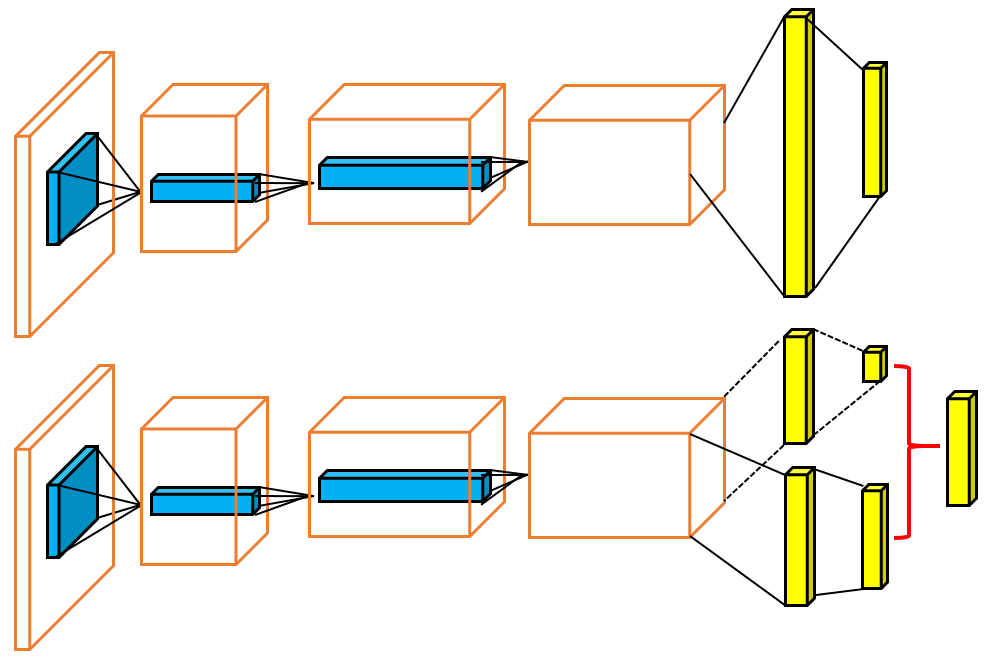
\includegraphics[scale=0.5]{static/dueling.png}
  \caption{普通网络结构与Dueling-Net结构}
\end{figure}

如下图所示,第一个模型为一般的DQN神经网络结构,第二个为Dueling-Net的网络结构。DQN网络结构输入层接入若干个卷积层,然后是全连接层,输出当前状态下对应动作的Q值。而Dueling-Net会将卷积层提取的特征分为两路,上路的输出代表当前环境本身就具备的价值$V(s)$;下路的输出代表当前状态下每个Action能够带来的额外价值。最后两路会在此汇聚到一起得到每个动作的Q值。Dueling-Net能学到环境本身具有的价值。
\chapter{游戏控制设计}
在本课题中,控制agent可分为两个过程:
\begin{enumerate}
  \item 用现实网络去玩游戏 (play)
  \item 对目标网络进行更新 (update)
\end{enumerate}
\section{游戏运行环境}
OpenAI Gym 是一个可以用于开发强化学习的工具库,提供python接口,可以方便编写强化学习并提供环境接口运行。
OpenAI Gym主要包含:
\begin{itemize}
  \item Gym 开源: 包含许多经典的游戏环境控制接口,这些接口有相同的名称以及传入参数,方便开发者设计强化和开发学习算法并进行实验比较,这些经典的游戏包括Atari和CartPole等。
  \item Gym service:为用户对训练算法性能的比较提供API接口,方便评价算法的性能。
\end{itemize}
本课题采用Christian Kauten开源的gym扩展\href{https://github.com/Kautenja/gym-super-mario-bros}{gym-super-mario-bros}\cite{gym-super-mario-bros}。
\begin{figure}
  \centering
  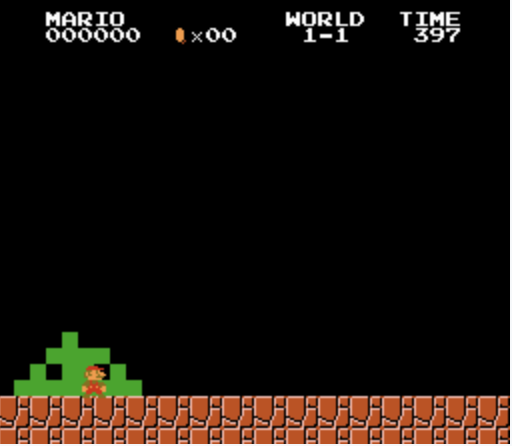
\includegraphics[scale=0.5]{static/mario.png}
  \caption{gym-super-mario-bros游戏界面}
\end{figure}
安装如下:
\begin{lstlisting}[language={bash}]
  pip install gym-super-mario-bros
\end{lstlisting}
使用示例如下:
\cleardoublepage
\begin{lstlisting}[language={python}, caption={super-mario控制}]
from nes_py.wrappers import BinarySpaceToDiscreteSpaceEnv
import gym_super_mario_bros
from gym_super_mario_bros.actions import SIMPLE_MOVEMENT
env = gym_super_mario_bros.make('SuperMarioBros-v0')
env = BinarySpaceToDiscreteSpaceEnv(env, SIMPLE_MOVEMENT)

done = True
for step in range(5000):
    if done:
        state = env.reset()
    state, reward, done, info = env.step(env.action_space.sample())
    env.render()

env.close()
\end{lstlisting}


\section{输入输出}
在游戏的每一个状态(画面像素帧),输入为超级马里奥最近4个画面像素帧的灰度图像。使用最近4个画面是为了让模型学习到当前马里奥的状态(高度,速度,移动方向等等)以及敌人的运动状态。为了使计算机更加容易理解计算机中的画面,使用超级玛丽北京为黑色的环境,这样原本背景的蓝天白云的噪声将不会产生影响。
每一个状态经过现实网络模型的输出为当前超级马里奥可以选择执行的动作,包括上下左右,跳跃,以及这些动作的组合:
\begin{lstlisting}[language={python}]
SIMPLE_MOVEMENT = [
  ['NOOP'],
  ['right'],
  ['right', 'A'],
  ['right', 'B'],
  ['right', 'A', 'B'],
  ['A'],
  ['left'],
]
\end{lstlisting}
\section{Reward以及目标}
本游戏的$reward$有以下公式确定:
\begin{equation}
  reward = V + C + D
\end{equation}
\begin{itemize}
  \item $V$:马里奥上一个状态与当前状态的不同水平位置的差,$V<0$ 代表agent向左走,$V>0$代表agent向右走。
  \item $C$:马里奥上一个状态与当前状态的时间差,代表马里奥在上一个状态到当前状态花了多长时间。
  \item $D$:马里奥是否在上一个状态执行动作后死亡,如果死亡$D=-15$,如果没死$D=0$。
\end{itemize}

$reward$最终会归一化为[-1,1]的范围。

\textbf{本算法控制游戏进行的首要目标为:控制游戏人物每一个回合在没有死亡的情况下,尽可能运动到水平位置距离起点远的位置。}
\section{游戏控制算法}
整个游戏控制算法由DQN算法及其三大改进构成,与传统DQN不同之处在于:
为了减少DQN出现过估计的情况,Q值更新公式采用Double DQN(\ref{alg:double-dqn});
  经验回放时,为了平衡不同样本表现得比率,使网络能够更快的学习到新知识,抽样方法采取Experienced Replay;
  为了使神经网络更深入理解环境本身的价值与动作在环境产生的额外价值,价值神经网络结构采用Dueling-Net的结构。

为了减少画面中原本存在的干扰和加快神经网络的处理速度,会对每一个输入的画面图像有一个预处理过程:
\begin{itemize}
  \item 裁剪掉图像上方对机器来说无意义的信息如分数,生命值,时间值等;
  \item 由于图像较大占用内存过多,因此对其进行缩放为(200*200)的大小;
  \item 将游戏的北京画面改为黑色背景,减少背景产生的干扰。
\end{itemize}

算法描述如算法(\ref{alg:mario})所示:
\begin{algorithm}
  \caption{超级玛丽控制算法}
  \begin{algorithmic}[1]
    \State 初始化Dueling-net网络参数
    \State 初始化经验库memory大小,memory\_size,经验库采用SumTree结构
    \State 初始化游戏,进入状态 s
    \While{经验库没存满}
    \State 随机选择当前状态下能选择的动作a
    \State 执行动作a,到达新的状态s',并获得环境的反馈r
    \State 将状态转化过程<s,a,r,s'>存到经验库memory,更新经验库
    \State 更新状态s $\gets$ s'
    \EndWhile
    \State 设置游戏进行学习的回合总数n
    \State 设置网络更新频率freq
    \State 设置网络的学习频率learning\_freq
    \For{i in range(n)}
    \State 获取当前的状态s
    \State $s_i$作为q-eval网络的输入,得到输出的动作$a_i$
    \State 执行动作$s_i$,到达新的状态$s_{i+1}$,并获得环境的反馈$r_i$
    \State 将状态转化过程$<s_i,a_i,r_i,s_{i+1}>$存到经验库memory,更新经验库 
    \If{i\% freq == 0}
    \State 将q-eval网络的参数更新到q-target网络
    \EndIf
    \If{i \% learning\_freq == 0}
    \State 从经验库中获取优先级最高的经验$<s_j,a_j,r_j,s_{j+1}>$
    \State q-eval网络从经验中$<s_j,a_j,r_j,s_{j+1}>$学习,更新参数
    \EndIf
    \EndFor
  \end{algorithmic}
  \label{alg:mario}
\end{algorithm}
\begin{figure}
  \centering
  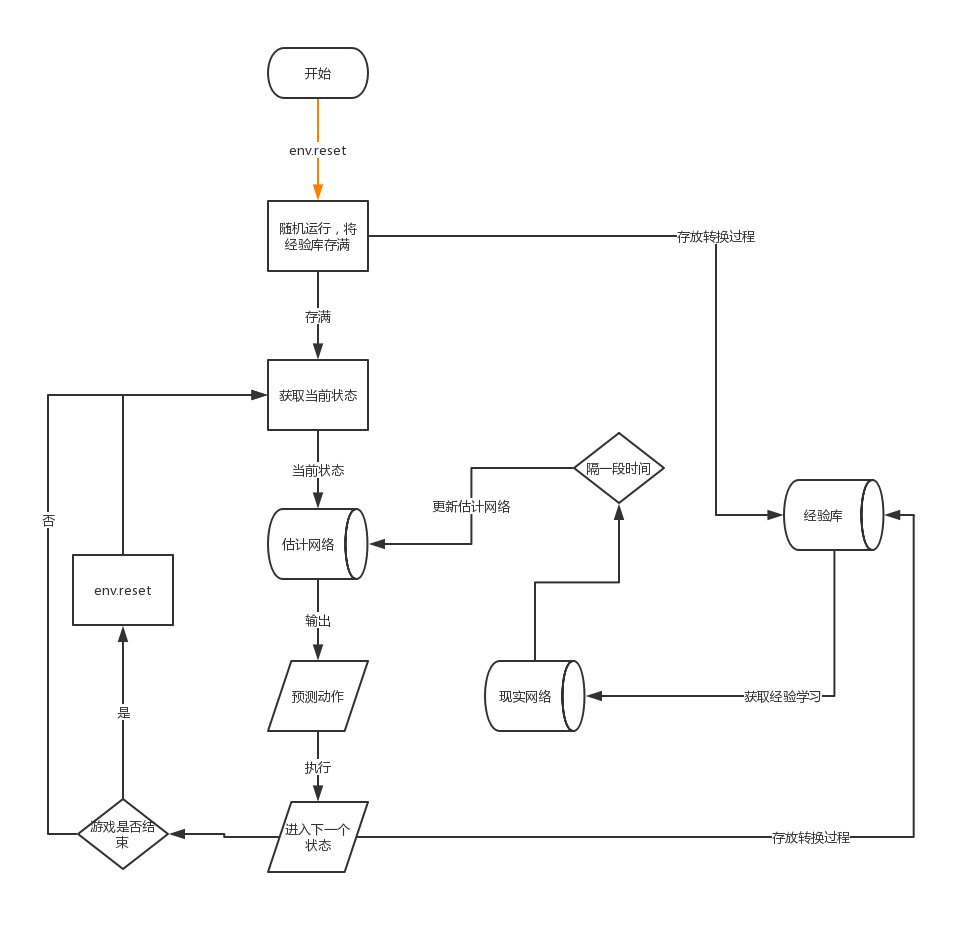
\includegraphics[scale=0.4]{static/graph.png}
  \caption{算法控制过程流程图}
\end{figure}
\cleardoublepage

\section{网络模型结构}

网络结构图如(\ref{fig:net})所示,输入为(32,4,200,200)大小的图片,其中32是batch\_size的大小,经过经过三个卷积层,每个卷积层的激活函数为Relu,然后是池化操作。卷积处理完成之后经过线性连接层分别得到网络输出的动作值以及当前状态的advantage。下面是网络结构每一层从输入到输出的具体结构:
\begin{enumerate}
  \item 输入:输入为(32,4,200,200)大小,其中32是批处理的batch\_size大小
  \item 卷积层:卷积核大小为8,步幅长度为4,经过激励函数为Relu,然后经过池化层,最后单个处理的输出为(32,24,24)
  \item 卷积层:卷积核大小为4,步幅长度大小为2,,经过激励函数Relu,然后进行池化操作,最后单个输出为(64,5,5)
  \item 卷积层:卷积核大小为2,步幅长度大小为2,经过激励函数Relu,然后进行池化操作,最后单个输出为(128,2,2)
  \item 卷积之后连接到两个不同的全连接层:
  \begin{enumerate}
    \item value连接层,输入为2*2*128,中间含有一个大小为128隐藏层,输入为1,即当前环境的价值
    \item advantage连接层,输入为2*2*128,中间含有一个大小为512的隐藏层,输出个数为动作总数,表示每个动作当前的优势值
  \end{enumerate}
  \item 最终输出:$value+(advantage-mean(advantage))$
\end{enumerate}
\begin{figure}
  \centering
  \caption{超级玛丽控制所使用的网络结构}
  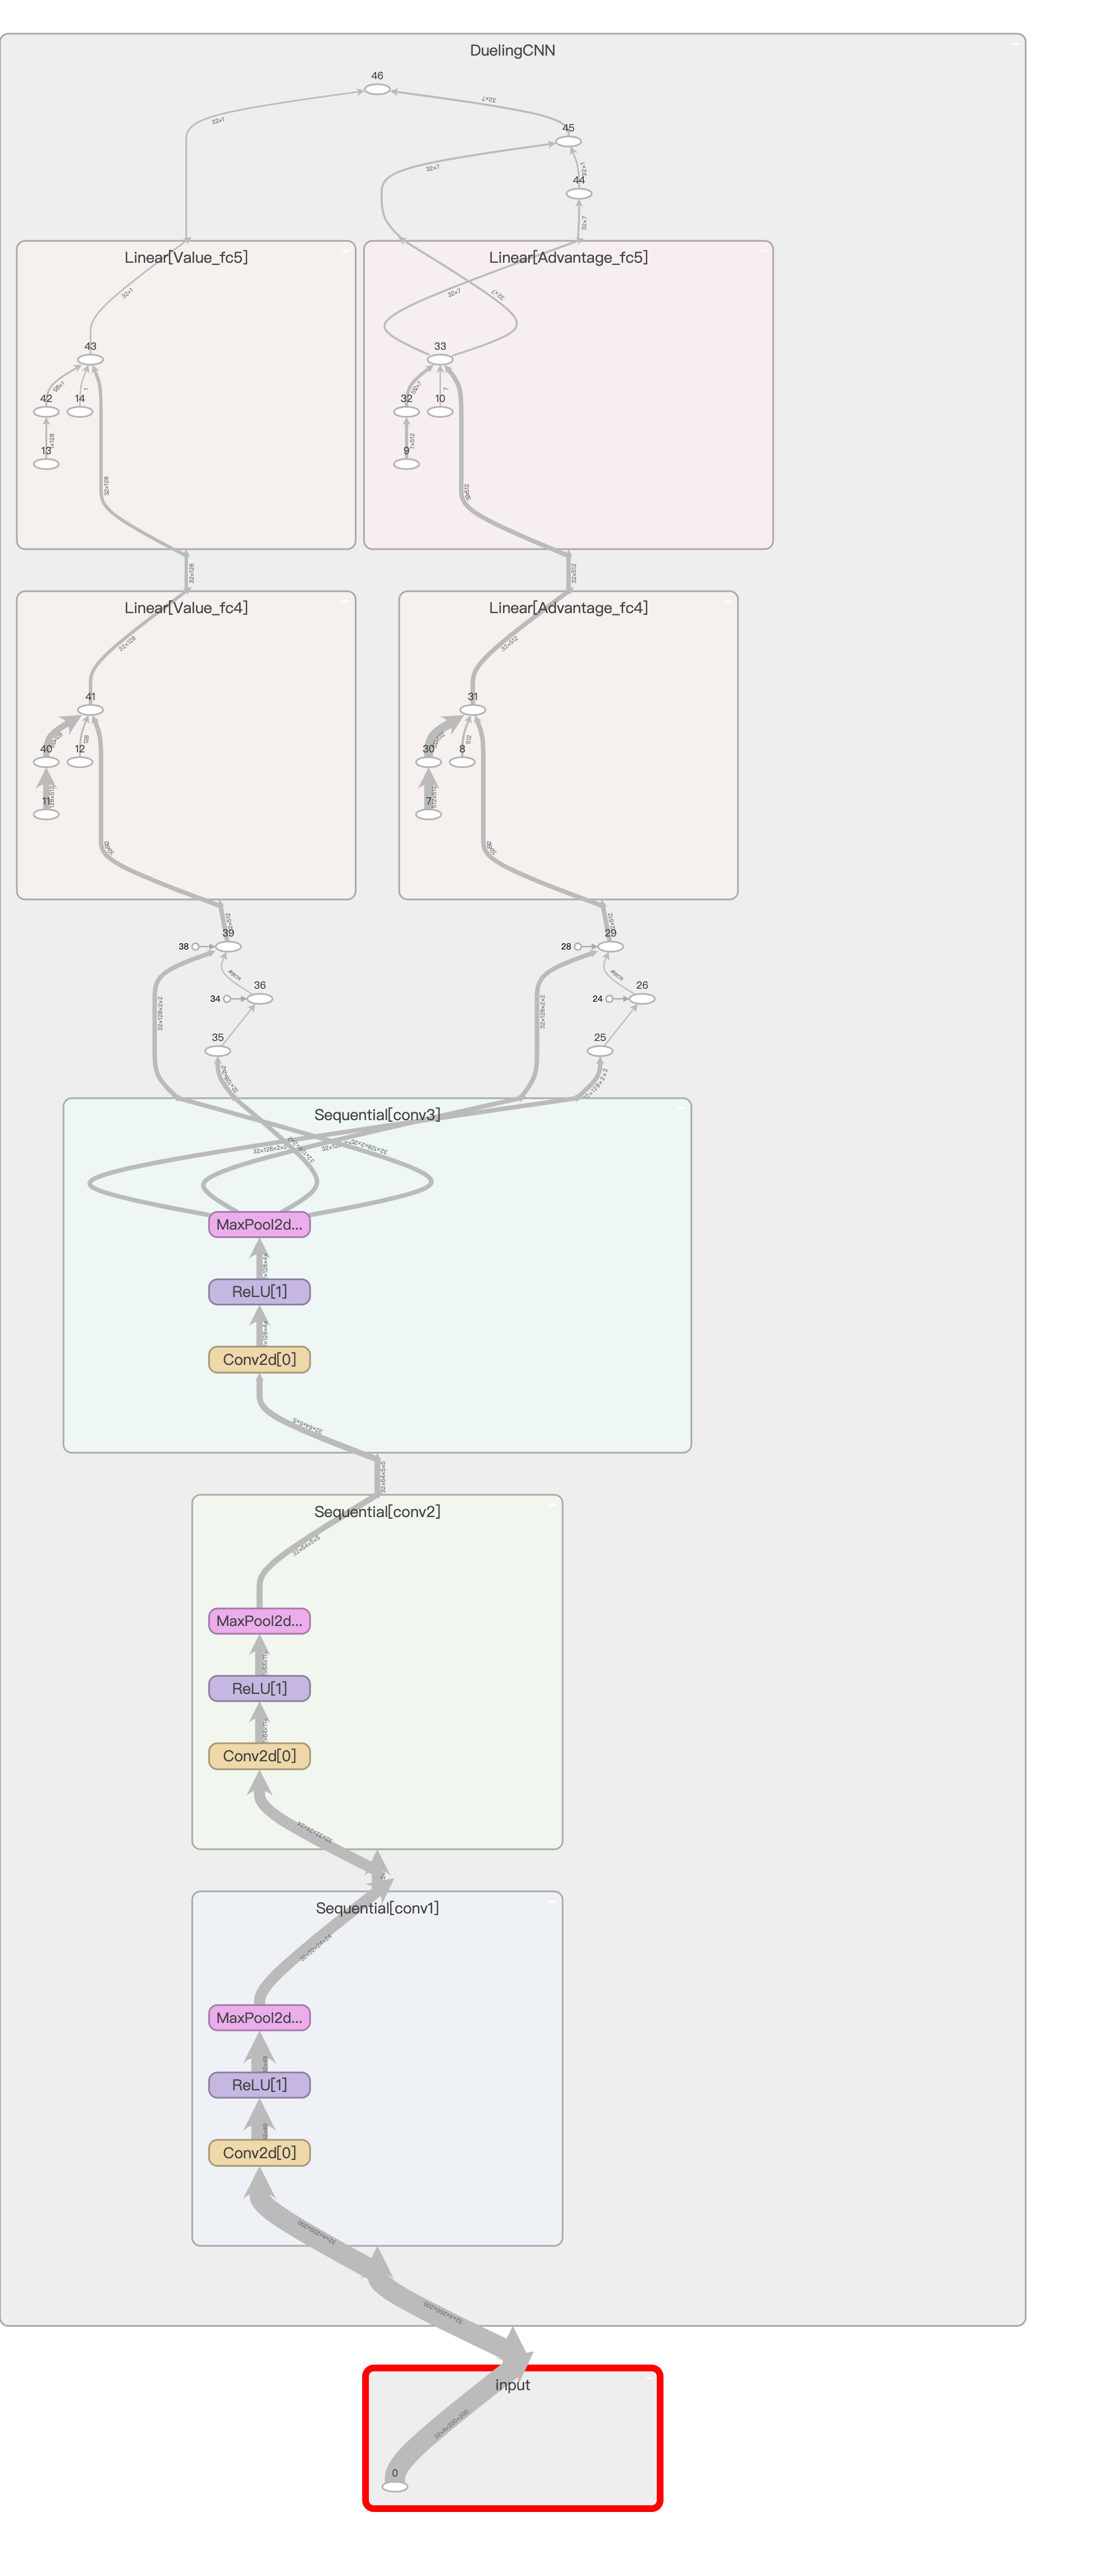
\includegraphics[width=500pt,height=700pt]{static/dueling_net.png}
  \label{fig:net}
\end{figure}
\cleardoublepage
\section{游戏控制的难点}
\begin{figure}[!htp]
  \centering
  \begin{subfigure}{3cm}
      \centering
      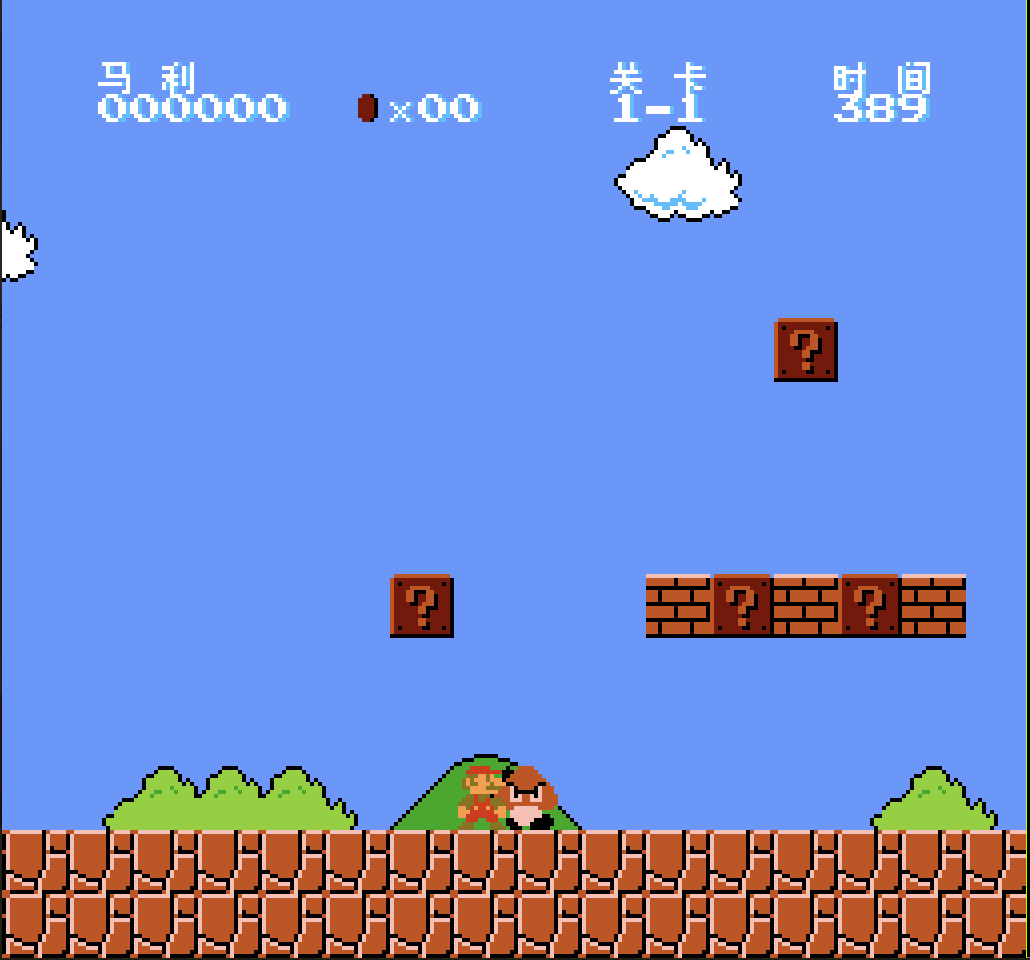
\includegraphics[height=3cm]{static/a.png}
      \caption{遇到第一个NPC}
  \end{subfigure}
  \hspace{1em}
  \begin{subfigure}{3cm}
    \centering
    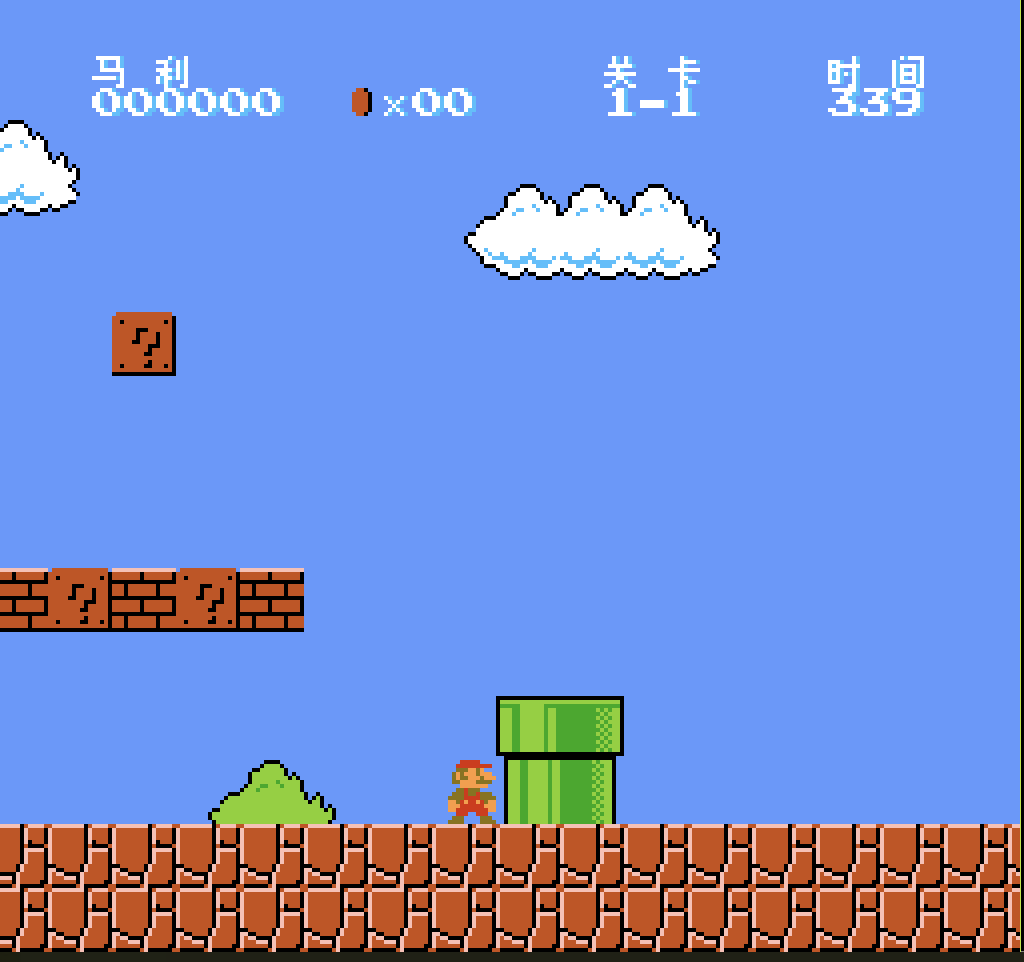
\includegraphics[height=3cm]{static/b.png}
    \caption{遇到第一个水管}
  \end{subfigure}
  \hspace{1em}
  \begin{subfigure}{3cm}
    \centering
    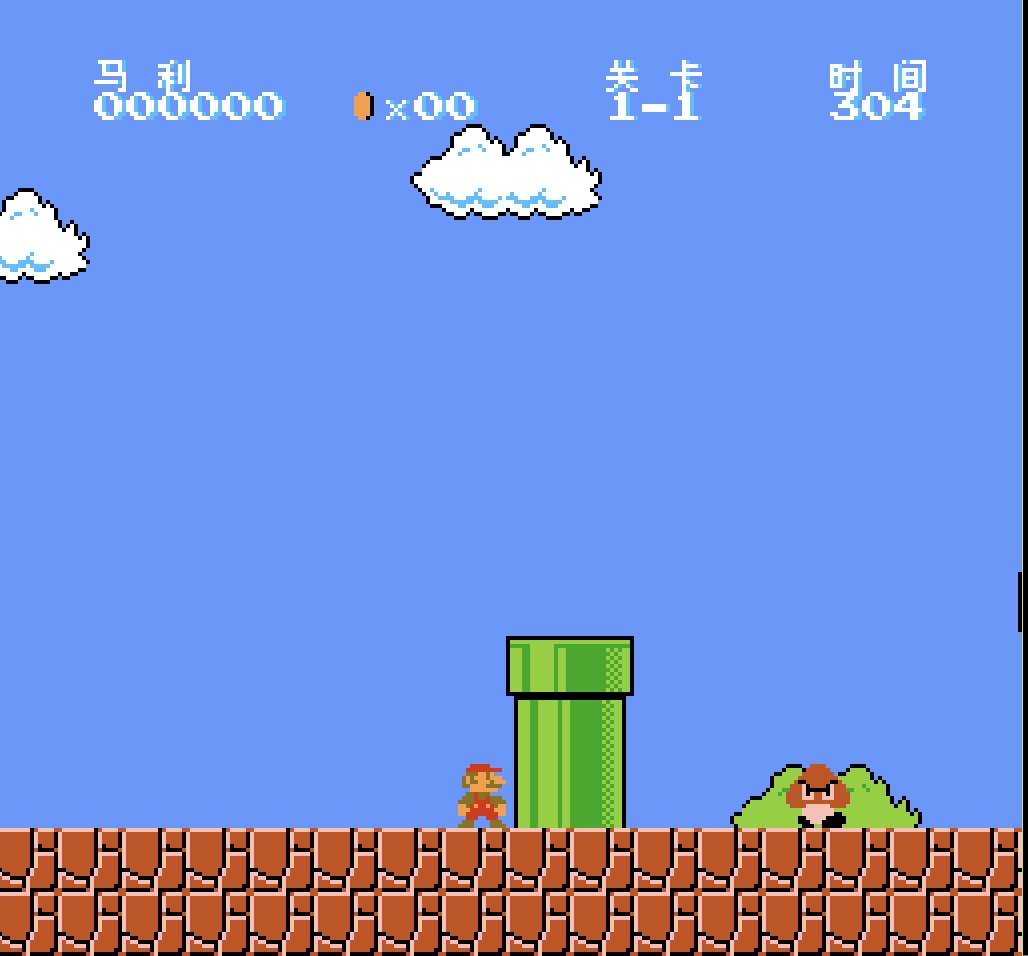
\includegraphics[height=3cm]{static/c.png}
    \caption{遇到比较高的水管}
  \end{subfigure}
  \hspace{1em}
  \begin{subfigure}{3cm}
    \centering
    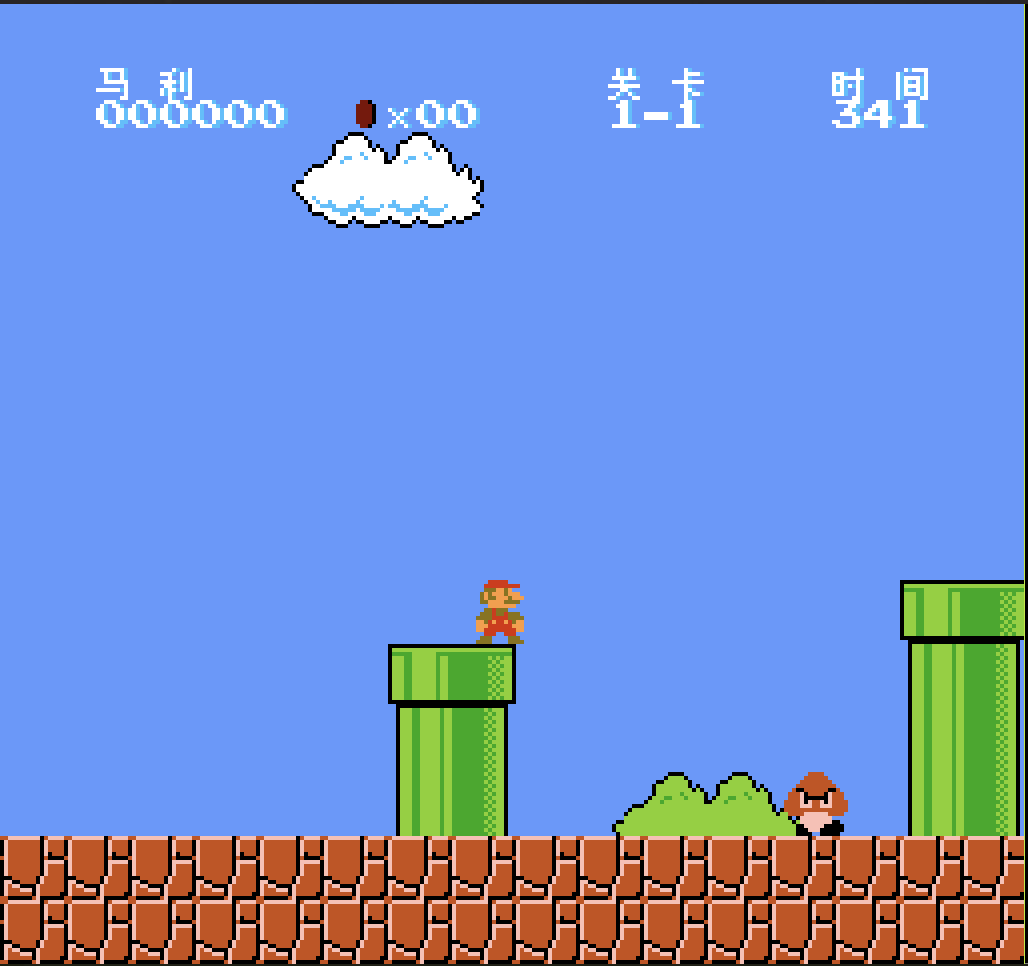
\includegraphics[height=3cm]{static/d.png}
    \caption{跳下水管}
  \end{subfigure}

  \begin{subfigure}{3cm}
      \centering
      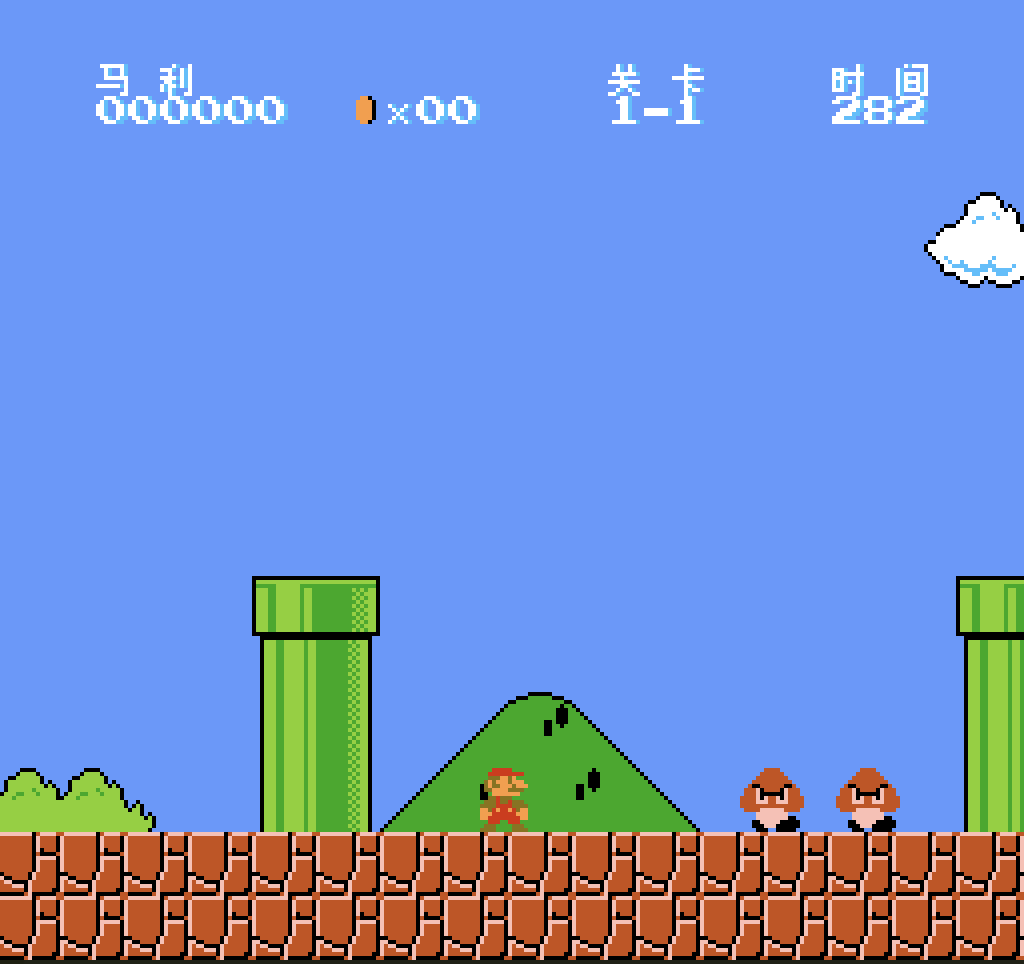
\includegraphics[height=3cm]{static/e.png}
      \caption{遇到最高的水管}
  \end{subfigure}
  \hspace{1em}
  \begin{subfigure}{3cm}
    \centering
    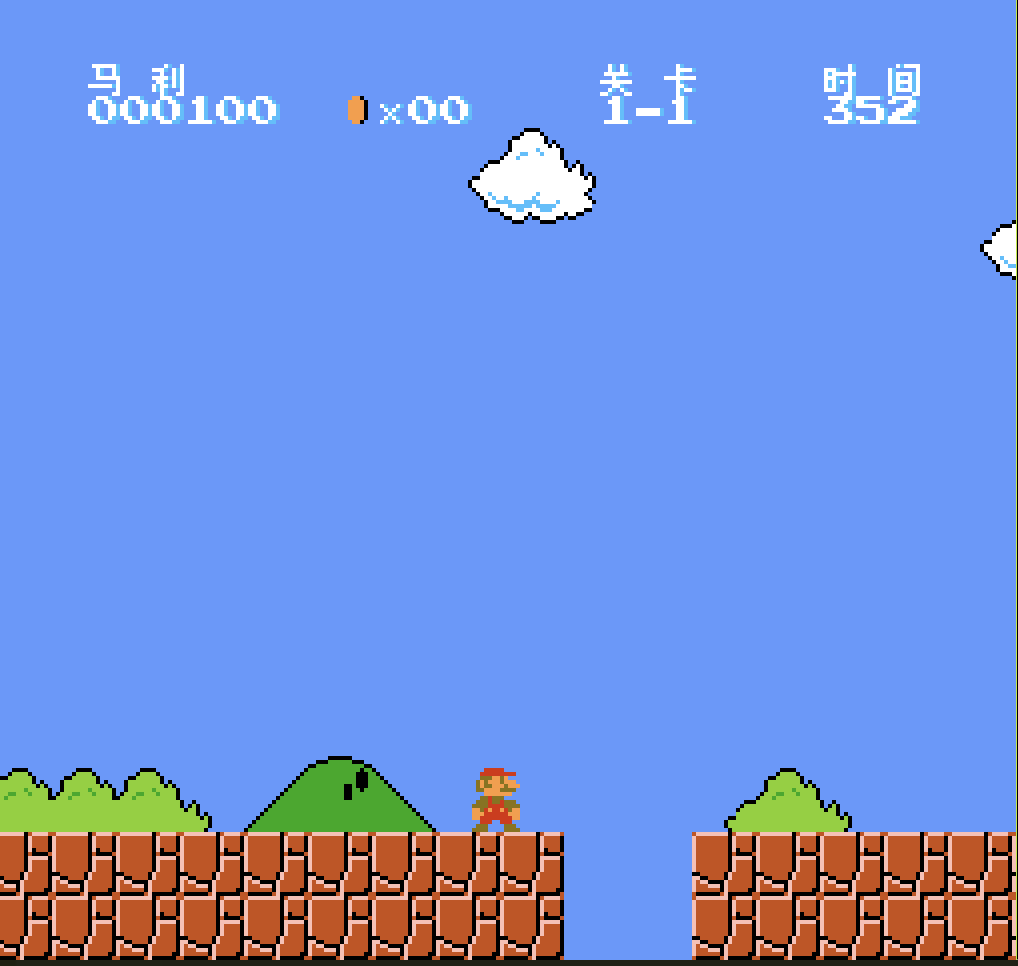
\includegraphics[height=3cm]{static/f.png}
    \caption{遇到第一个坑}
  \end{subfigure}
  \hspace{1em}
  \begin{subfigure}{3cm}
    \centering
    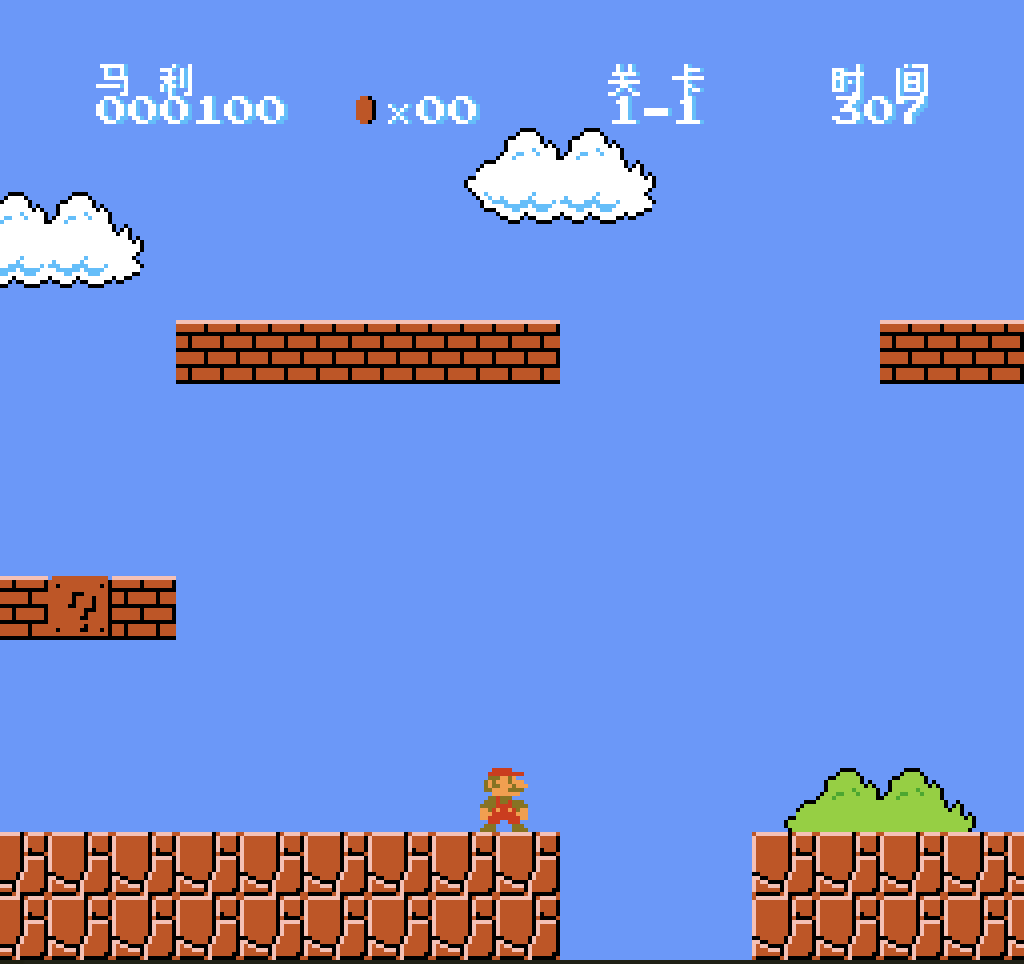
\includegraphics[height=3cm]{static/g.png}
    \caption{遇到第二个坑}
  \end{subfigure}
  \hspace{1em}
  \begin{subfigure}{3cm}
    \centering
    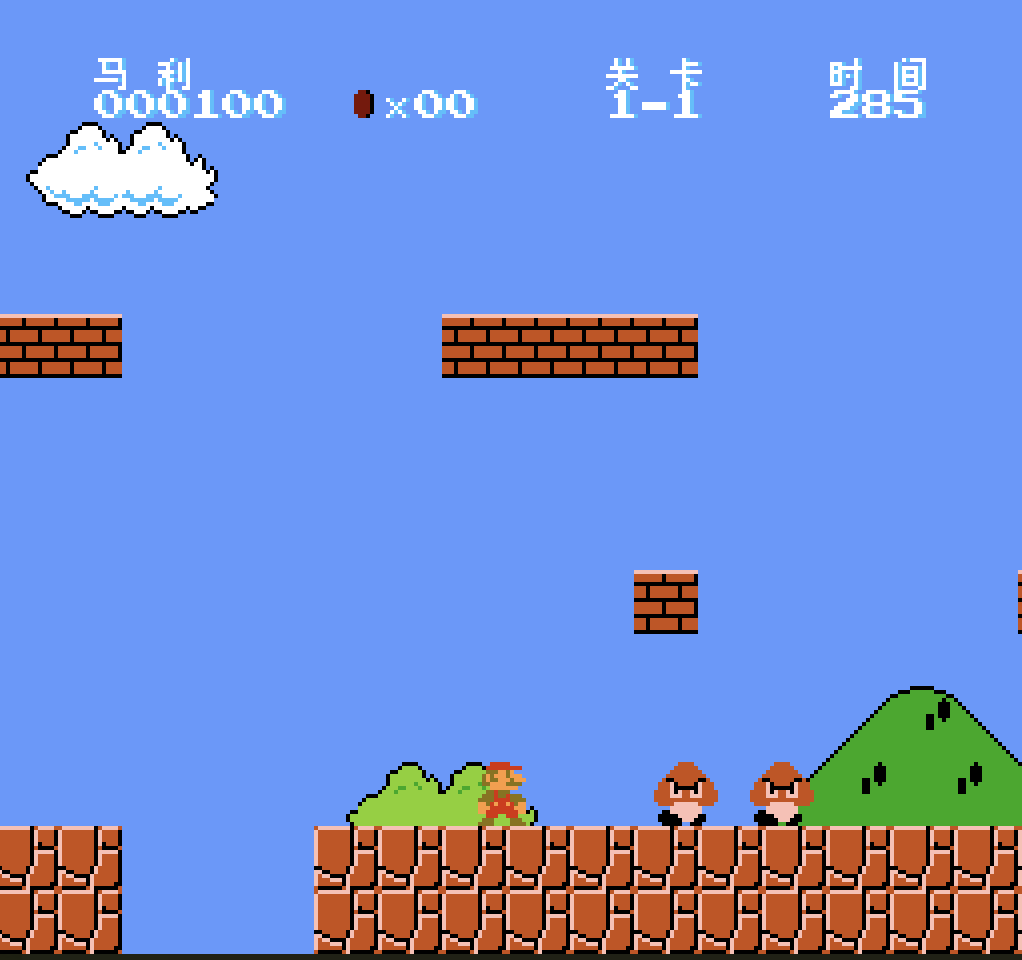
\includegraphics[height=3cm]{static/h.png}
    \caption{跳过坑后遇到NPC}
  \end{subfigure}
  \begin{subfigure}{3cm}
      \centering
      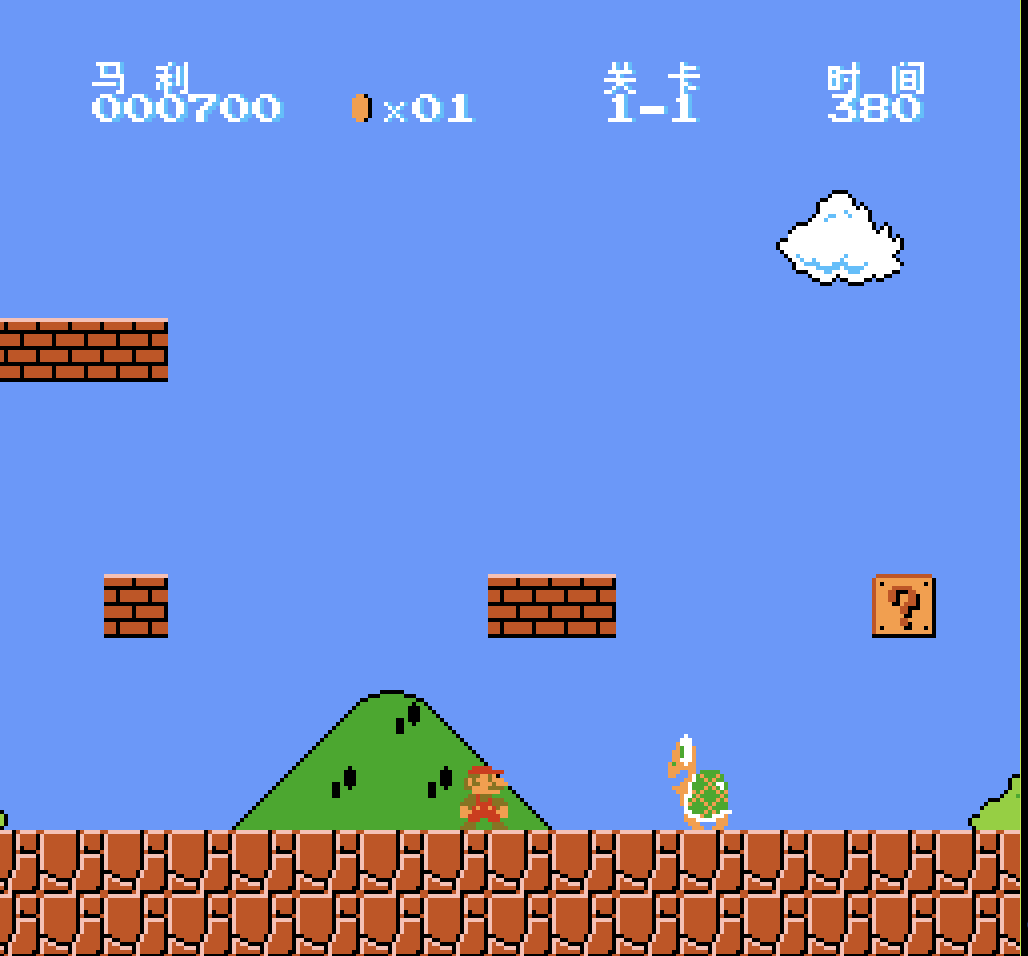
\includegraphics[height=3cm]{static/i.png}
      \caption{跳跃刚结束遇到NPC}
  \end{subfigure}
  \hspace{1em}
  \begin{subfigure}{3cm}
    \centering
    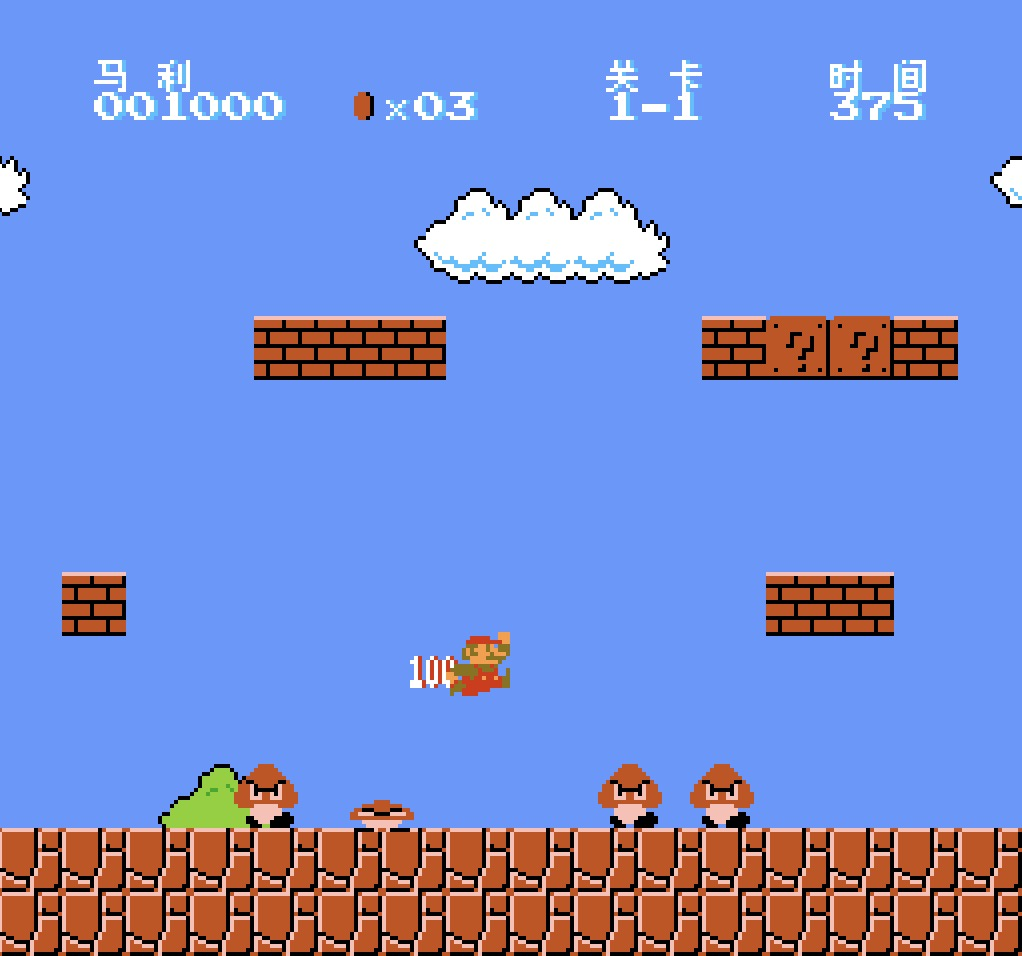
\includegraphics[height=3cm]{static/j.png}
    \caption{最难的点}
  \end{subfigure}
  \hspace{1em}
  \begin{subfigure}{3cm}
    \centering
    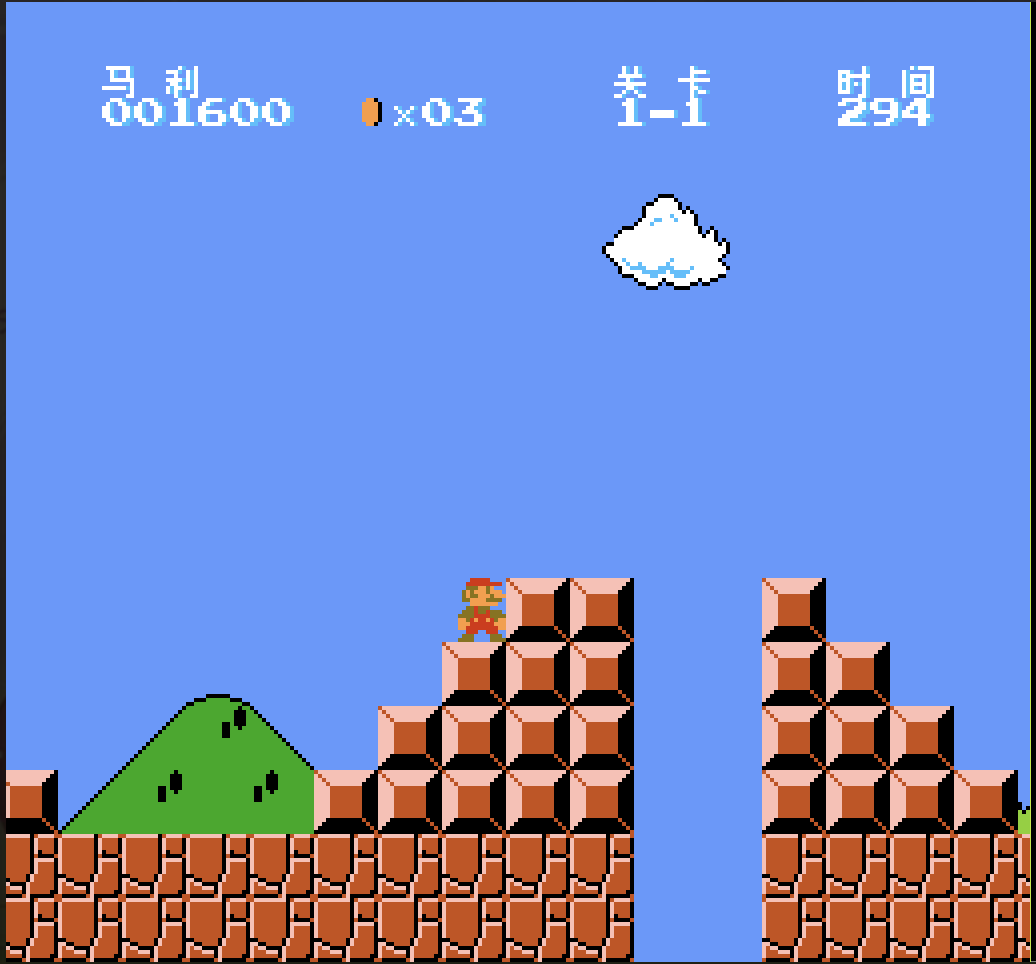
\includegraphics[height=3cm]{static/l.png}
    \caption{最后一个坑}
  \end{subfigure}
  \hspace{1em}
  \begin{subfigure}{3cm}
    \centering
    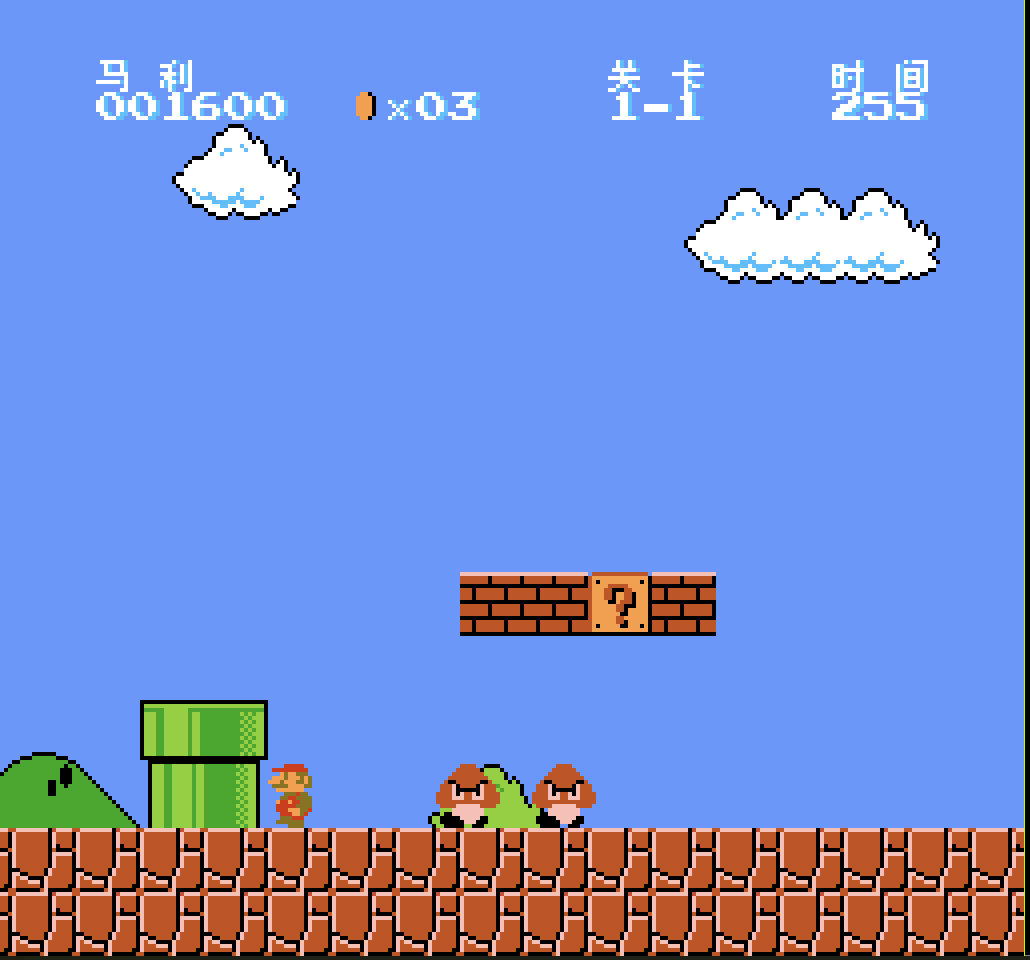
\includegraphics[height=3cm]{static/m.png}
    \caption{最后遇到的NPC}
  \end{subfigure}
  \label{fig:mario}
  \caption{超级玛丽在游戏中的难点}
\end{figure}
\cleardoublepage

由上图游戏的画面,我们可以看到,控制超级玛丽向前运动存在很多处的难点,甚至许多处难点人类来控制也无法做到死亡。在这个游戏当中,对于笔者本身的硬件环境来说,确实很难做到完美。下面是关于这些难点的详细介绍,通过介绍这些难点,可以更加清晰地认识到算法在控制模型做决策时的难易程度:在每个时刻,算法都需要做出以下决策:
\begin{enumerate*}
  \item 当游戏人物处于游戏中任意一个画面时,水平方向选择向左还是向右;
  \item 当游戏人物处于地面上,为了获得更高的奖励,是否需要跳跃;
  \item 如果做出跳跃的决策,应该跳多高(持续多长时间);
  \item 在跳跃的过程中是否做水平移动,向哪个方向做水平移动;
  \item 在跳跃的时候如果移动,应该水平移动多远(持续移动多久)。
\end{enumerate*}
这些决策某个时刻做出,会在不久之后影响后面的状态,有的影响甚至无法挽回。以下将举几个图片的例子来详细说明:
\begin{exmp}[遇到水管]
  在遇到水管的时候,神经网络应该做出决策,决定超级玛丽应该跳多高才能跳过水管,在跳过水管的那一个时刻应该决定向右。
\end{exmp}
\begin{exmp}[跳下水管]
  在跳下水管的时候应该考虑是在什么时机跳下不会遇到NPC而死亡,如果跳的时机不对,刚好遇到NPC,那么这个决策就很失败。
\end{exmp}
\begin{exmp}[遇到深坑]
  遇到深坑的时候,需要决策的更加复杂,坑的宽度不一样,需要跳跃的高度以及跳跃时移动的位置也不一样,如果跳的过早这会掉入坑里,跳的过晚则会直接走到坑里;水平移动的距离太短会导致死亡,水平移动的距离太长则会在落到地上的时刻直接遇到NPC来不及闪躲。
\end{exmp}
\begin{exmp}[遇到NPC]
  在遇到NPC的时候决策是最难的,这个时候需要注意的是可能会遇到不止一个NPC决策,如图j,在遇到NPC需要决定何时跳跃,跳跃落下来的时候会很容易遇到另一个NPC来不及进行第二次跳跃而导致死亡。因此,在实验数据中,在这个位置的动作选择是最难的。
\end{exmp}

\chapter{实验结果与分析}
\section{实验结果}
\begin{figure}[!htp]
    \centering
    \begin{subfigure}{6cm}
        \centering
        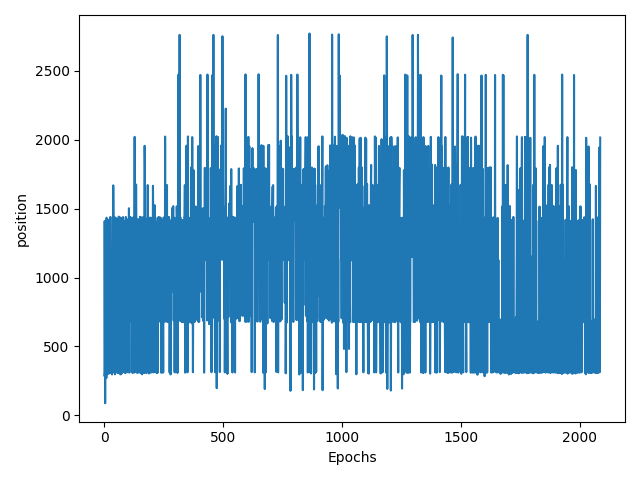
\includegraphics[height=6cm]{static/reword.png}
        \caption{超级玛丽每回合结束的位置}
    \end{subfigure}
    \hspace{4em}
    \begin{subfigure}{6cm}
      \centering
      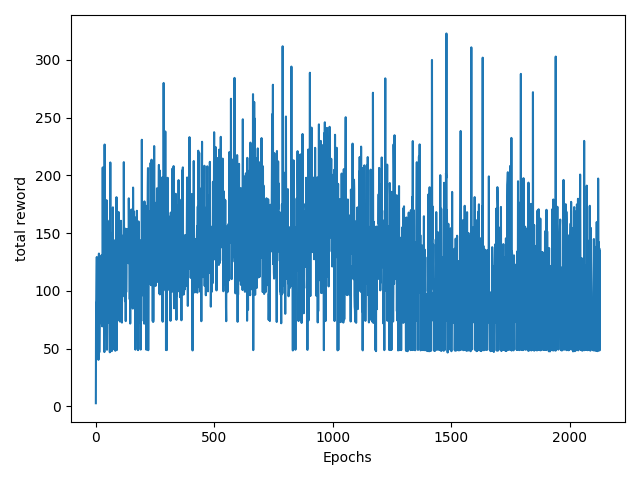
\includegraphics[height=6cm]{static/myplot.png}
      \caption{超级玛丽每回合的奖励和}
    \end{subfigure}
    \bicaption{实验数据表现}{}
    \label{fig:data}
\end{figure}
由游戏过程的数据图\ref{fig:data}可以发现以下几个特点:
\begin{enumerate}
    \item 当游戏在进行前250个回合,学习效果不是很好,处于尝试错误并积累经验的阶段,没有明显的进步。
    \item 当游戏250回合到接近1500回合,游戏人物已经有了明显的学习成果,在能稳定运动到700以上的水平距离。
    \item 在500到1500回合,游戏人物死亡距离稳定提高到了2000的位置(j的位置),网络学习的表现也是最好的。
    \item 在250回合之后,游戏人物通过2500(最后一个难点)的位置,已经有了明显的进步。
    \item 在1500回合之后,算法的表现出现了下滑,网络学习到的东西开始朝着反方向发展,表现越来越差。 
\end{enumerate}

在第一幅数据图中,可以看出,游戏人物死亡的位置明显出现了阶段点,如250,750,接近1500,1750,2000,2500的位置。这些位置都是DQN算法表现得不够好的地方。算法在这些地方表现不够好是DQN本身的特点所导致的。首先DQN算法是基于价值的算法,DQN过分关注眼前的利益,因此会很容易忽略当前的动作会对之后的状态产生的影响。例如在某一时刻选择一个动作在当时可能是能带来瞬间价值最大化的,当时选择了这个动作有可能会对后面的状态产生不好的影响。这就好像贪图了眼前的蝇头小利,往往会错失更大的利益。DQN算法看不到更长远的利益,这也是算法需要进行改进的方面。
\section{结论}
DQN算法与三大改进算法的结合成功应用到了超级玛丽这款游戏上。本课题所采取的算法取得了预期的学习效果,算法模型会根据不同的环境状态采取预期的动作:当游戏人物遇到水管时会做出向右跳跃的决策;当遇上较高的水管时会选择持续向上跳直到到达水管顶部,然后再向右走;当人物遇到NPC时会做出跳跃来躲避的决策;当遇到深坑的情况下,会在合适的位置跳跃;当任务向右走遇到阻挡物的时候会改变动作执行跳跃。

然而在一些比较复杂的情况下,网络模型目前做出的判断依然不够智能:当遇到相当多的NPC的时候,模型此时决策的跳跃位置不是非常准确,导致落地的时刻来不及躲避新的NPC;跳跃的持续时间还不能精确掌握,导致还无法完美一次性跳跃障碍水管。随着训练不断地持续下去,网络模型参数的更新可能会朝着不好的方向发展,还无法做到稳定单调不减。DQN算法还不能做到看到长远的结果而改变目前的策略。

随着训练的进行,大量回合的训练,神经网络学习到的干扰越来越强,学习效果也会因此开始逐渐变差。在游戏控制的后期阶段,已经出现明显的成绩降低,因此采取措施使得学习效果能够保持单调不减是下一步需要重点改进的地方。

\section{需要改进的地方}
由于笔者的当前硬件有限,因此无法将图像识别部分的网络模型做的足够精确,网络模型的识别精确度有限。其次,经验库的大小memory size相对而言比较小,因此在学习过程中存在学习的经验效率低下的问题。最后是游戏的环境存在环境相对于其他游戏来说,逻辑复杂,场景变化较多,输出动作过多,导致神经网络并不能很准确的分类出当前应当做出的动作。因此总结需要改进的地方有以下几点:
\begin{itemize}
    \item 提升计算机硬件水平,加速训练效果。
    \item 提升经验库的容量或者无损压缩经验库存放的转化关系。
    \item 使用更加强大的卷积神经网络结构,对游戏画面图像的分类更加精确。
    \item 游戏画面预处理,突出游戏当前的重要状态,减少游戏环境的噪声干扰
    \item 精简游戏逻辑,使用更简单的动作,比如舍去向左走的动作。
    \item 评估奖励机制的不合理之处,做出相应改进。
    \item 改进算法,机器不再只关心当前的利益,更应该关心长远的影响,比如使用基于策略的方法,或者使用Actor-Critic的方法。
\end{itemize}
\chapter{总结}
本文介绍了深度强化学习的发展与目前的研究内容,重点介绍了DQN算法及其三大改进:double DQN,Prioritized Experience Replay DQN,Prioritized,Dueling DQN。其中double DQN是关于DQN公式(更新方法)的改进,Prioritized Experience Replay是关于经验回放的改进,Dueling DQN是关于神经网络结构的改进。
在本课题中,笔者成功将DQN算法及其三大改进算法结合起来应用到超级玛丽这款经典游戏的控制上,取得了明显的学习效果。
在取得了明显的学习效果中,还存在着许多不足之处,如收敛不够,神经网络分类不准确,对于长期的价值掌握不够等。还需要在这些方面做进一步改进。通过本次课题对深度强化学习有了充分的认知理解,掌握了DQN算法背后所蕴含的思想,深度学习的发展带领人工智能向前迈进了一大步。深度强化学习无论是在理论上还是在实际应用中都有着巨大的前景,目前深度强化学习还有很广阔的发展空间。
\chapter*{致谢}
四年的大学学习生活在即将划上一个句号,而于我的人生来说却仅仅只是一个逗号,我将面对新的征程的开始。本研究及论文是在我的导师李辉的亲切关怀和耐心的指导下完成的。我还要感谢一下一起完成毕业论文小组的同学们,如果没有你们的支持和倾心的协助,我是无法解决这些困难和疑惑,最终能够让本文顺利完成。至此论文付梓之际,我的心情无法保持平静,从开始选择课题到论文的顺利完成,有无数可敬的师长、朋友给了我很多的帮助,在这里请您接受我诚挚的谢意! 谢谢我的女友帮我画图,因为有她我才能从容完成这份论文的撰写。大学四年时间是如此短暂,四年中我不仅认识了一群好朋友、好同学,更幸运地遇上了一大批兢兢业业教导我们的老师,感谢有你们的时光。在未来的职业生涯中我也将牢牢铭记你们的谆谆教导,铭记母校教给我的一切。
\printbibliography[heading=bibintoc]

% \include{tex/intro}
% \include{tex/example}
% \include{tex/faq}
% \chapter{总结}
本文介绍了深度强化学习的发展与目前的研究内容,重点介绍了DQN算法及其三大改进:double DQN,Prioritized Experience Replay DQN,Prioritized,Dueling DQN。其中double DQN是关于DQN公式(更新方法)的改进,Prioritized Experience Replay是关于经验回放的改进,Dueling DQN是关于神经网络结构的改进。
在本课题中,笔者成功将DQN算法及其三大改进算法结合起来应用到超级玛丽这款经典游戏的控制上,取得了明显的学习效果。
在取得了明显的学习效果中,还存在着许多不足之处,如收敛不够,神经网络分类不准确,对于长期的价值掌握不够等。还需要在这些方面做进一步改进。通过本次课题对深度强化学习有了充分的认知理解,掌握了DQN算法背后所蕴含的思想,深度学习的发展带领人工智能向前迈进了一大步。深度强化学习无论是在理论上还是在实际应用中都有着巨大的前景,目前深度强化学习还有很广阔的发展空间。

% \appendix % 使用英文字母对附录编号

% 附录内容,本科学位论文可以用翻译的文献替代。
% %# -*- coding: utf-8-unix -*-
% !TEX program = xelatex
% !TEX root = ../thesis.tex
% !TEX encoding = UTF-8 Unicode
\chapter{搭建模板编译环境}

\section{安装TeX发行版}

\subsection{Mac OS X}

Mac用户可以从MacTeX主页\footnote{\url{https://tug.org/mactex/}}下载MacTeX。
也可以通过brew包管理器\footnote{\url{http://caskroom.io}}安装MacTeX。

\begin{lstlisting}[basicstyle=\small\ttfamily, numbers=none]
brew cask install mactex
\end{lstlisting}

\subsection{Linux}

建议Linux用户使用TeXLive主页\footnote{\url{https://www.tug.org/texlive/}}的脚本来安装TeXLive。
以下命令将把TeXLive发行版安装到当前用户的家目录下。
若计划安装一个供系统上所有用户使用的TeXLive,请使用root账户操作。

\begin{lstlisting}[basicstyle=\small\ttfamily, numbers=none]
wget http://mirror.ctan.org/systems/texlive/tlnet/install-tl-unx.tar.gz
tar xzvpf install-tl-unx.tar.gz
cd install-tl-20150411/
./install-tl
\end{lstlisting}

\section{安装中文字体}

\subsection{Mac OS X、Deepin}

Mac和Deepin用户双击字体文件即可安装字体。

\subsection{RedHat/CentOS用户}

RedHat/CentOS用户请先将字体文件复制到字体目录下,调用fc-cache刷新缓存后即可在TeXLive中使用新字体。

\begin{lstlisting}[basicstyle=\small\ttfamily, numbers=none]
mkdir ~/.fonts
cp *.ttf ~/.fonts				# 当前用户可用新字体
cp *.ttf /usr/share/fonts/local/	# 所有用户可以使用新字体
fc-cache -f
\end{lstlisting}


% \include{tex/app_eq}
% \include{tex/app_cjk}
% %# -*- coding: utf-8-unix -*-
% !TEX program = xelatex
% !TEX root = ../thesis.tex
% !TEX encoding = UTF-8 Unicode
\chapter{模板更新记录}
\label{chap:updatelog}

\textbf{2018年1月} v0.10发布,项目转移至 \href{https://github.com/sjtug/SJTUThesis}{SJTUG} 名下,并增加了英文模版,修改了默认字体设置。

\textbf{2016年12月} v0.9.5发布,改用GB7714-2015参考文献风格。

\textbf{2016年11月} v0.9.4发布,增加算法和流程图。

\textbf{2015年6月19日} v0.9发布,适配ctex 2.x宏包,需要使用TeXLive 2015编译。

\textbf{2015年3月15日} v0.8发布,使用biber/biblatex组合替代 \BibTeX ,带来更强大稳定的参考文献处理能力;添加enumitem宏包增强列表环境控制能力;完善宏包文字描述。

\textbf{2015年2月15日} v0.7发布,增加盲审选项,调用外部工具插入扫描件。

\textbf{2015年2月14日} v0.6.5发布,修正一些小问题,缩减git仓库体积,仓库由sjtu-thesis-template-latex更名为SJTUThesis。

\textbf{2014年12月17日} v0.6发布,学士、硕士、博士学位论文模板合并在了一起。

\textbf{2013年5月26日} v0.5.3发布,更正subsubsection格式错误,这个错误导致如"1.1 小结"这样的标题没有被正确加粗。

\textbf{2012年12月27日} v0.5.2发布,更正拼写错误。在diss.tex加入ack.tex。

\textbf{2012年12月21日} v0.5.1发布,在 \LaTeX 命令和中文字符之间留了空格,在Makefile中增加release功能。

\textbf{2012年12月5日} v0.5发布,修改说明文件的措辞,更正Makefile文件,使用metalog宏包替换xltxtra宏包,使用mathtools宏包替换amsmath宏包,移除了所有CJKtilde(\verb+~+)符号。

\textbf{2012年5月30日} v0.4发布,包含交大学士、硕士、博士学位论文模板。模板在\href{https://github.com/sjtug/SJTUThesis}{github}上管理和更新。

\textbf{2010年12月5日} v0.3a发布,移植到 \XeTeX/\LaTeX 上。

\textbf{2009年12月25日} v0.2a发布,模板由CASthesis改名为sjtumaster。在diss.tex中可以方便地改变正文字号、切换但双面打印。增加了不编号的一章“全文总结”。
添加了可伸缩符号(等号、箭头)的例子,增加了长标题换行的例子。

\textbf{2009年11月20日} v0.1c发布,增加了Linux下使用ctex宏包的注意事项、.bib条目的规范要求,
修正了ctexbook与listings共同使用时的断页错误。

\textbf{2009年11月13日} v0.1b发布,完善了模板使用说明,增加了定理环境、并列子图、三线表格的例子。

\textbf{2009年11月12日} 上海交通大学硕士学位论文 \LaTeX 模板发布,版本0.1a。



\backmatter % 文后无编号部分

% 参考资料


% 致谢、发表论文、申请专利、参与项目、简历
% 用于盲审的论文需隐去致谢、发表论文、申请专利、参与的项目
\makeatletter

\ifsjtu@coursepaper
\else

  % "研究生学位论文送盲审印刷格式的统一要求"
  % http://www.gs.sjtu.edu.cn/inform/3/2015/20151120_123928_738.htm

  % 盲审删去删去致谢页
  \ifsjtu@review\relax\else
    % %# -*- coding: utf-8-unix -*-
% !TEX program = xelatex
% !TEX root = ../thesis.tex
% !TEX encoding = UTF-8 Unicode
\begin{thanks}

  感谢所有测试和使用交大学位论文 \LaTeX 模板的同学!

  感谢那位最先制作出博士学位论文 \LaTeX 模板的交大物理系同学!

  感谢William Wang同学对模板移植做出的巨大贡献!
  
  感谢 \href{https://github.com/weijianwen}{@weijianwen} 学长一直以来的开发和维护工作!
  
  感谢 \href{https://github.com/sjtug}{@sjtug} 以及 \href{https://github.com/dyweb}{@dyweb} 对 0.9.5 之后版本的开发和维护工作!
  
  感谢所有为模板贡献过代码的同学们, 以及所有测试和使用模板的各位同学!

\end{thanks}
         % 致谢
  \fi

  % \ifsjtu@bachelor
  %   % 学士学位论文要求在最后有一个英文大摘要,单独编页码
  %   % \include{tex/end_english_abstract}
  % \else
  %   % 盲审论文中,发表学术论文及参与科研情况等仅以第几作者注明即可,不要出现作者或他人姓名
  %   \ifsjtu@review\relax
  %     \include{tex/pubreview}
  %     \include{tex/projectsreview}
  %   \else
  %     \include{tex/pub}       % 发表论文
  %     \include{tex/projects}  % 参与的项目
  %     % \include{tex/patents}   % 申请专利
  %     \include{tex/resume}    % 个人简历
  %   \fi
  % \fi
\fi

\makeatother

\end{document}
